\mfpicnumber{1}

\opengraphsfile{FunctionArithmetic}

\setcounter{footnote}{0}

\label{FunctionArithmetic}

As we mentioned in Section \ref{GraphsofFunctions}, in this chapter, we are studying functions in a more abstract and general setting.  In this section, we begin our study of what can be considered as the \textit{algebra of functions}  by defining \textit{function arithmetic.}  

\smallskip


Given two real numbers,  we have four primary arithmetic operations available to us:  addition, subtraction, multiplication, and division (provided we don't divide by $0$.)  Since the functions we study in this text have ranges which are sets of real numbers, it makes sense we can extend these arithmetic notions to functions. 

\smallskip

For example,  to add two functions means  we add their outputs;  to subtract two functions, we subtract their outputs, and so on and so forth.  More formally, given two functions $f$ and $g$, we \textit{define} a new function $f+g$ whose rule is determined by adding the outputs of $f$ and $g$.  That is $(f+g)(x) = f(x) + g(x)$.  While  this looks suspiciously like some kind of distributive property, it is nothing of the sort.  The `$+$' sign in the expression `$f+g$' is part of the \textit{name} of the function we are defining,\footnote{We could have just as easily called this new function $S(x)$ for `sum' of $f$ and $g$ and defined $S$ by $S(x) = f(x) + g(x)$.} whereas the plus sign `$+$' sign in the expression $f(x) + g(x)$ represents real number addition: we are adding the output from $f$, $f(x)$ with the output from $g$, $g(x)$ to determine the output from the sum function, $(f+g)(x)$.

\smallskip

 Of course, in order to define $(f+g)(x)$ by the formula $(f+g)(x) = f(x) + g(x)$, both $f(x)$ and $g(x)$ need to be defined in the first place; that is, $x$ must be in the domain of $f$ \textit{and} the domain of $g$.  You'll recall\footnote{see Section \ref{AppSetTheory}.} this means $x$ must be in the \textit{intersection} of the domains of $f$ and $g$.   We define the following.
 
 \smallskip

\colorbox{ResultColor}{\bbm

\begin{defn}  \label{functionarithmeticdefn}  \index{function ! arithmetic} Suppose $f$ and $g$ are functions and $x$ is in both the domain of $f$ and the domain of $g$.
\begin{itemize}

\item  The \index{function ! sum} \textbf{sum} of $f$ and $g$, denoted $f+g$, is the function defined by the formula \[(f+g)(x) = f(x) + g(x)\]

\item  The \index{function ! difference} \textbf{difference} of $f$ and $g$, denoted $f-g$, is the function defined by the formula \[(f-g)(x) = f(x) - g(x)\]

\item  The \index{function ! product} \textbf{product} of $f$ and $g$, denoted $fg$, is the function defined by the formula \[(fg)(x) = f(x)g(x)\]

\item  The \index{function ! quotient} \textbf{quotient} of $f$ and $g$, denoted $\dfrac{f}{g}$, is the function defined by the formula \[\left(\dfrac{f}{g}\right)(x) = \dfrac{f(x)}{g(x)},\] provided $g(x) \neq 0$.


\end{itemize}

\end{defn}

\ebm}

\medskip



We put these definitions to work for us in the next example.


\begin{ex}  \label{funcarithex} Consider the following functions:

\begin{multicols}{2}

\begin{itemize}

\item  $f(x) = 6x^2 - 2x$ \vphantom{$g(t) = 3-\dfrac{1}{t}$, $t > 0$.}

\item $g(t) = 3-\dfrac{1}{t}$, $t > 0$

\end{itemize}

\end{multicols}

\begin{multicols}{2}

\begin{itemize}

\item  $h = \{ (-3,2), (-2,0.4), (0,\sqrt{2}), (3, -6) \}$  

\item  $s$ whose graph is given below:

\end{itemize}

\end{multicols}


\begin{center}

\begin{mfpic}[15]{-2}{5}{-3}{4}
\axes
\tlabel[cc](5,-0.5){\scriptsize $t$}
\tlabel[cc](0.5,4){\scriptsize $y$}
\xmarks{-1, 0, 1, 2, 3, 4}
\ymarks{-2, -1, 0, 1, 2, 3}
\tcaption{\scriptsize $y = s(t)$}
\tlpointsep{4pt}
\scriptsize
\tlabel[cc](1, -2.5){$(0,-2)$}
\tlabel[cc](2, 0.5){$(1,0)$}
\tlabel[cc](2, 2.5){$(2,2)$}
\tlabel[cc](-2, -2.5){$(-2, -2)$}
\axislabels {x}{{$-1 \hspace{7pt}$} -1,{$1$} 1, {$2$} 2, {$3$} 3, {$4$} 4}
\axislabels {y}{{$2$} 2,{$-1$} -1,{$1$} 1, {$3$} 3}
\normalsize
\penwd{1.25pt}
 \arrow \polyline{(-2, -2), (0, -2), (2, 2), (5, 2)}
\point[4pt]{(-2,-2), (0,-2), (1,0), (2,2)}
\end{mfpic}

 
\end{center}

\begin{enumerate}

\item  \label{funcarithfindvaluesex} Find and simplify the following function values:

\begin{multicols}{4}

\begin{enumerate}

\item  $(f+g)(1)$ \vphantom{ $\left( \dfrac{s}{h} \right)(0)$}

\item $(s-f)(-1)$ \vphantom{ $\left( \dfrac{s}{h} \right)(0)$}

\item $(fg)(2)$ \vphantom{ $\left( \dfrac{s}{h} \right)(0)$}

\item  $\left( \dfrac{s}{h} \right)(0)$

\setcounter{HW}{\value{enumii}}

\end{enumerate}

\end{multicols}


\begin{multicols}{4}

\begin{enumerate}

\setcounter{enumii}{\value{HW}}

\item \label{threefunctionsfirstex} $((s+g)+h)(3)$  \vphantom{$\left(\dfrac{f+g}{s}\right)(3)$}

\item $(s+(g+h))(3)$  \vphantom{$\left(\dfrac{f+g}{s}\right)(3)$}

\item $\left(\dfrac{f+h}{s}\right)(3)$

\item  \label{threefunctionslastex} $(f(g-h))(-2)$ \vphantom{$\left(\dfrac{f+g}{s}\right)(3)$}

\end{enumerate}

\end{multicols}

\item  Find the domain of each of the following functions:

\begin{multicols}{2}

\begin{enumerate}

\item $hg$

\item  $\dfrac{f}{s}$

\end{enumerate}

\end{multicols}

\item \label{arithexpressionex} Find expressions for the functions below.  State the domain for each.

\begin{multicols}{2}

\begin{enumerate}

\item   \label{proddomainex} $(fg)(x)$

\item  \label{quotdomainex}  $\left(\dfrac{g}{f}\right)(t)$

\end{enumerate}

\end{multicols}

\end{enumerate}

{\bf Solution.}  

\begin{enumerate}

\item \begin{enumerate}

\item  By definition, $(f+g)(1) = f(1) + g(1)$.   We find $f(1) = 6(1)^2-2(1) = 4$ and $g(1) = 3 - \frac{1}{1} = 2$. So we get  $(f+g)(1) = 4+2 = 6$.

\item  To find $(s-f)(-1) = s(-1) - f(-1)$, we need both $s(-1)$ and $f(-1)$.  To get $s(-1)$, we look to the graph of $y = s(t)$ and look for the $y$-coordinate of the point on the graph with the $t$-coordinate of $-1$.  While not labeled directly, we infer the point $(-1,-2)$ is on the graph which means $s(-1) = -2$. For $f(-1)$, we compute: $f(-1) = 6(-1)^2-2(-1) = 8$.  Putting it all together, we get $(s-f)(-1) = (-2) -(8) = -10$.

\item Since $(fg)(2) = f(2)g(2)$, we first  compute $f(2)$ and $g(2)$. We find $f(2) = 6(2)^2-2(2) = 20$ and $g(2) = 2 + \frac{1}{2} = \frac{5}{2}$, so $(fg)(2) = f(2) g(2) = (20)\left(\frac{5}{2}\right) = 50$.

\item By definition, $\left( \frac{s}{h} \right)(0) = \frac{s(0)}{h(0)}$.  Since $(0, -2)$ is on the graph of $y=s(t)$, so we know $s(0)  = -2$.  Likewise, the ordered pair $(0, \sqrt{2}) \in h$, so $h(0) = \sqrt{2}$.  We get  $\left( \frac{s}{h} \right)(0) = \frac{s(0)}{h(0)} = \frac{-2}{\sqrt{2}} = -\sqrt{2}$.

\item  The expression $((s+g)+h)(3)$ involves \textit{three} functions.  Fortunately, they are grouped so that we can apply Definition \ref{functionarithmeticdefn} by first considering the sum of the two functions $(s+g)$ and $h$, then to the sum of the two functions $s$ and $g$: $((s+g)+h)(3) = (s+g)(3)+h(3) = (s(3)+g(3))+h(3)$.  To get $s(3)$, we look to the graph of $y = s(t)$.  We infer the point $(3,2)$ is on the graph of $s$, so $s(3) = 2$.  We compute $g(3) = 3-\frac{1}{3} = \frac{8}{3}$.  To find $h(3)$, we note $(3, -6) \in h$, so $h(3) = -6$.  Hence, $((s+g)+h)(3) = (s+g)(3)+h(3) = (s(3)+g(3))+h(3) = \left(2+\frac{8}{3}\right) + (-6) = -\frac{4}{3}$.

\item The expression   $(s+(g+h))(3)$ is very similar to the previous problem, $((s+g)+h)(3)$ except that the $g$ and $h$ are grouped together here instead of the $s$ and $g$.  We proceed as above applying Definition \ref{functionarithmeticdefn} twice and find $(s+(g+h))(3) = s(3) + (g+h)(3) = s(3)+(g(3)+h(3))$.  Substituting the values for $s(3)$, $g(3)$ and $h(3)$, we get   $(s+(g+h))(3) = 2 + \left(\frac{8}{3} + (-6)\right)  = -\frac{4}{3}$, which, not surprisingly, matches our answer to the previous problem.

\item  Once again, we find the expression  $\left(\frac{f+h}{s}\right)(3)$ has more than two functions involved.  As with all fractions, we treat `$-$' as a grouping symbol and interpret  $\left(\frac{f+h}{s}\right)(3) = \frac{(f+h)(3)}{s(3)} = \frac{f(3)+h(3)}{s(3)}$.  We compute $f(3) = 6(3)^2-2(3) = 48$ and have $h(3) = -6$ and $s(3) = 2$ from above.  Hence, $\left(\frac{f+h}{s}\right)(3) =  \frac{f(3)+h(3)}{s(3)} = \frac{48+(-6)}{2} = 21$.

\item We need to need to exercise caution in parsing $(f(g-h))(-2)$.  In this context, $f$, $g$, and $h$ are all functions, so we interpret $(f(g-h))$ as the function and $-2$ as the argument. We view the function $f(g-h)$ as the product of $f$ and the function $g-h$.  Hence, $(f(g-h))(-2) = f(-2) [(g-h)(-2)] = f(-2) [g(-2) - h(-2)]$.  We compute $f(-2) = 6(-2)^2-2(-2) = 28$, and $g(-2)= 3 - \frac{1}{-2} = 3 + \frac{1}{2} = \frac{7}{2} = 3.5$.  Since $(-2, 0.4) \in h$, $h(-2) = 0.4$.  Putting this altogether, we get $(f(g-h))(-2) = f(-2) [(g-h)(-2)] = f(-2) [g(-2) - h(-2)] = 28(3.5-0.4) = 28(3.1) = 86.8$.

\end{enumerate}

\item \begin{enumerate}

\item To find the domain of $hg$, we need to find the real numbers in both the domain of $h$ and the domain of $g$.  The domain of $h$ is $\{ -3, -2, 0, 3 \}$ and the domain of $g$ is $\{ t \in \mathbb{R} \, | \, t > 0 \}$ so the only real number in common here is $3$.  Hence, the domain of $hg$ is $\{ 3\}$, which may be small, but it's better than nothing.\footnote{Since $(hg)(3) = h(3)g(3) = (-6)\left(\frac{8}{3}\right) = -16$, we can write $hg = \{ (3,-16) \}$.}

\item To find the domain of $\frac{f}{s}$, we first note the domain of $f$ is all real numbers, but that the domain of $s$, based on the graph, is just $[-2, \infty)$.  Moreover, $s(t) = 0$ when $t=1$, so we must exclude this value from the domain of $\frac{f}{s}$.  Hence, we are left with $[-2, 1) \cup (1, \infty)$.

\end{enumerate}

\item  

\begin{enumerate}

\item  By definition, $(fg)(x) = f(x)g(x)$.  We are given $f(x) = 6x^2-2x$ and $g(t) = 3 - \frac{1}{t}$ so $g(x) = 3 - \frac{1}{x}$.  Hence, 

\[ \begin{array}{rclr}


(fg)(x) & = & f(x)g(x) & \\
           & = &  \left( 6x^2-2x \right) \left( 3 - \dfrac{1}{x} \right) & \\
           & = &  18x^2 - 6x^2 \left(\dfrac{1}{x}\right) - 2x(3) + 2x \left(\dfrac{1}{x}\right)  & \text{distribute} \\
           & = & 18x^2 - 6x - 6x + 2 & \\
           & = & 18x^2 - 12x + 2 & \\ \end{array} \]
           
To find the domain of $fg$, we note the domain of $f$ is all real numbers, $(-\infty, \infty)$ whereas the domain of $g$ is restricted to $\{ t \in \mathbb{R} \, | \, t > 0 \} = (0, \infty)$.  Hence, the domain of $fg$ is likewise restricted to $(0, \infty)$.  Note if we relied solely on the \textbf{simplified formula} for $(fg)(x) = 18x^2 - 12x + 2$, we would have obtained the \textit{incorrect} answer for the domains of $fg$.  

\item To find an expression for $\left(\frac{g}{f}\right)(t) = \frac{f(t)}{g(t)}$ we first note $f(t) = 6t^2-2t$ and $g(t) = 3 - \frac{1}{t}$.  Hence:
\setlength{\extrarowheight}{12pt}

\begin{longtable}{rclr}
 
$\left( \dfrac{g}{f}\right)(t)$ & $=$ & $\dfrac{g(t)}{f(t)} $  & \\
& = & $\dfrac{3-\dfrac{1}{t}\vphantom{\left(\dfrac{1}{t}\right)}}{6t^2 - 2t}$ = $\dfrac{3-\dfrac{1}{t}\vphantom{\left(\dfrac{1}{t}\right)}}{6t^2 - 2t} \cdot \dfrac{t}{t}$ & simplify compound fractions  \\[.125in]

& = & $\dfrac{\left(3-\dfrac{1}{t}\right) t}{\left(6t^2 - 2t\right)t}$ =  $\dfrac{3t-1}{\left(6t^2 - 2t\right)t}$ & \\

& = & $\dfrac{3t-1}{2t^2(3t-1)}$ =  $\dfrac{\cancelto{1}{(3t-1)}}{2t^2\cancel{(3t-1)}}$ & factor and cancel \\

& = & $\dfrac{1}{2t^2}$ &  \\

\end{longtable} 

\setlength{\extrarowheight}{2pt}

Hence, $\left(\frac{g}{f} \right)(t) = \frac{1}{2t^2} = \frac{1}{2} t^{-2}$.  To find the domain of $\frac{g}{f}$, a real number must be both in the domain of $g$, $(0, \infty)$, and the domain of $f$, $(-\infty, \infty)$ so we start with the set $(0, \infty)$.  Additionally, we require $f(t) \neq 0$.  Solving $f(t) = 0$ amounts to solving $6t^2-2t = 0$ or $2t(3t-1) = 0$.  We find $t = 0$ or $t = \frac{1}{3}$ which means we need to exclude these values from the domain.  Hence, our final answer for the domain of $\frac{g}{f}$ is $\left(0, \frac{1}{3} \right) \cup \left(\frac{1}{3}, \infty \right)$.  Note that, once again,  using the  \textit{simplified formula} for $\left(\frac{g}{f}\right)(t)$ to determine the domain of $\frac{g}{f}$, would have produced erroneous results. \qed

\end{enumerate}

\end{enumerate}

\end{ex}
 
 A few remarks are in order.  First, in number \ref{funcarithfindvaluesex} parts \ref{threefunctionsfirstex} through \ref{threefunctionslastex}, we first encountered combinations of \textit{three} functions despite Definition \ref{functionarithmeticdefn} only addressing combinations of \textit{two} functions at a time.  It turns out that function arithmetic inherits many of the same properties of real number arithmetic. For example, we showed above that  $((s+g)+h)(3) = (s+(g+h))(3)$.  In general, given any three functions $f$, $g$, and $h$, $(f+g)+h = f +(g+h)$ that is, function addition is \textit{assocative}.  To see this, choose an element $x$ common to the domains of $f$, $g$, and $h$.  Then 
 
 \[ \begin{array}{rclr}
 
((f+g)+h)(x) & = & (f+g)(x)+h(x) & \text{definiton of $((f+g)+h)(x)$} \\

                    & = & (f(x)+g(x))+h(x) & \text{definition of $(f+g)(x)$} \\
                    & = & f(x) + (g(x)+h(x)) & \text{associative property of real number addition} \\
                    & = & f(x) + (g+h)(x) & \text{definition of $(g+h)(x)$} \\
                    & = & (f+(g+h))(x) & \text{definition of $(f+(g+h))(x)$} \\  \end{array} \]

The key step  to the argument is that  $(f(x)+g(x))+h(x)   =  f(x) + (g(x)+h(x))$ which is true courtesy of the associative property of real number addition.  And just like with real number addition, because function addition is associative, we may write $f+g+h$ instead of $(f+g)+h$ or $f+(g+h)$ even though, when it comes down to computations, we can only add two things together at a time.\footnote{Addition is a `binary' operation - meaning it is defined only on two objects at once.  Even though we write $1+2+3 = 6$,  mentally, we add just two of  numbers together at any given time to get our answer: for example, $1+2+3 = (1+2)+3 = 3+3 = 6$.}

\smallskip

For completeness, we summarize the properties of function arithmetic in the theorem below.  The proofs of the properties all follow along the same lines as the proof of the associative property and are left to the reader.  We investigate some additional properties in the exercises.

\smallskip

\colorbox{ResultColor}{\bbm

\begin{thm}  \label{functionarithmeticprops}  Suppose $f$, $g$ and $h$ are functions.

\begin{itemize}

\item   \textbf{Commutative Law of Addition:} $f+g =g+f$

\item  \textbf{Associative Law of Addition:} $(f+g) + h = f+(g+h)$

\item  \textbf{Additive Identity:}  The function $Z(x) = 0$ satisfies:  $f+Z = Z+f = f$ for all functions $f$.

\item  \textbf{Additive Inverse:}  The function $F(x) = -f(x)$ for all $x$ in the domain of $f$ satisfies:  \[ f+F=F+f=Z.\] 

\item  \textbf{Commutative Law of Multiplication:} $fg = gf$

\item  \textbf{Associative Law of Multiplication:} $(fg)h =f(gh)$

\item  \textbf{Multiplicative Identity:}  The function $I(x) = 1$ satisfies:  $fI = If = f$ for all functions $f$.

\item  \textbf{Multiplicative Inverse:}  If $f(x) \neq 0$ for all $x$ in the domain of $f$, then $F(x) = \dfrac{1}{f(x)}$ satisfies: \[ fF=Ff = I\]

\item  \textbf{Distributive Law of Multiplication over Addition:}  $f(g+h) = fg+fh$


\end{itemize}

\end{thm}

\ebm}

\smallskip

In the next example, we decompose given functions into sums, differences, products and/or quotients of other functions.  Note that there are infinitely many different ways to do this, including some trivial ones.  For example, suppose we were instructed to decompose $f(x) = x+2$ into a sum or difference of functions.  We could write $f = g+h$ where $g(x) = x$ and $h(x) = 2$ or we could choose $g(x) = 2x+3$ and $h(x) = -x-1$.  More simply, we could write $f = g+h$ where $g(x) = x+2$ and $h(x) = 0$.  We'll call this last decomposition a `trivial' decomposition.  Likewise, if we ask for a decomposition of $f(x) = 2x$ as a product, a nontrivial solution would be $f = gh$ where $g(x) = 2$ and $h(x) = x$ whereas a trivial solution would be $g(x) = 2x$ and $h(x) = 1$.  In general, non-trivial solutions to decomposition problems avoid using the additive identity, $0$,  for sums and differences and the multiplicative identity, $1$, for products and quotients.

\begin{ex} \label{funcarithdecompex}  

\begin{enumerate}

\item  For  $f(x) = x^2 - 2x$, find functions $g$, $h$ and $k$ to decompose $f$ nontrivially as:

\begin{multicols}{4}

\begin{enumerate}

\item  $f = g-h$

\item  $f = g+h$

\item  $f = gh$

\item  $f = g(h-k)$

\end{enumerate}

\end{multicols}

\item  For $F(t) = \dfrac{2t+1}{\sqrt{t^2-1}}$, find functions $G$, $H$ and $K$ to decompost $F$ nontrivially as:


\begin{multicols}{4}

\begin{enumerate}

\item  $F = \dfrac{G}{H}$ \vphantom{$F =  \dfrac{G+H}{K}$}

\item  $F = GH$ \vphantom{$F =  \dfrac{G+H}{K}$}

\item  $F = G+H$ \vphantom{$F =  \dfrac{G+H}{K}$}

\item  $F =  \dfrac{G+H}{K}$ 

\end{enumerate}

\end{multicols}


\end{enumerate}

{\bf Solution.}

\begin{enumerate}

\item 

\begin{enumerate}

\item To decompose $f = g-h$, we need functions $g$ and $h$ so $f(x) = (g-h)(x) = g(x) - h(x)$.  Given $f(x) = x^2 - 2x$,  one option is to let $g(x) = x^2$ and $h(x) = 2x$.  To check, we find $(g-h)(x) = g(x) - h(x) = x^2-2x = f(x)$ as required.  In addition to checking the formulas match up, we also need to check domains.  There isn't much work here since the domains of $g$ and $h$ are all real numbers which combine to give the domain of $f$ which is all real numbers.

\item  In order to write $f = g+h$, we need $f(x) = (g+h)(x) = g(x) + h(x)$.  One way to accomplish this is to write $f(x) = x^2 - 2x = x^2+(-2x)$ and identify $g(x) = x^2$ and $h(x)  = -2x$.  To check, $(g+h)(x) = g(x) + h(x) = x^2 - 2x = f(x)$.  Again, the domains for both $g$ and $h$ are all real numbers which combine to give $f$ its domain of all real numbers.

\item  To write $f = gh$, we require $f(x) = (gh)(x) = g(x) h(x)$.  In other words, we need to factor $f(x)$.  We find $f(x) = x^2-2x = x(x-2)$, so one choice is to select $g(x) = x$ and $h(x) = x-2$.  Then $(gh)(x) = g(x)h(x) = x(x-2) = x^2-2x = f(x)$, as required.  As above, the domains of $g$ and $h$ are all real numbers which combine to give $f$ the correct domain of $(-\infty, \infty)$.

\item  We need to be careful here interpreting the equation $f = g(h-k)$.  What we have is an equality of \textit{functions} so the parentheses here \textit{do not} represent function notation here, but, rather function \textit{multiplication}.  The way to parse $g(h-k)$, then, is the function $g$ \textit{times} the function $h-k$. Hence, we seek functions $g$, $h$, and $k$ so that $f(x) = [g(h-k)](x) = g(x) [(h-k)(x)] = g(x) (h(x) - k(x))$.    From the previous example, we know we can rewrite $f(x) = x(x-2)$, so one option is to set $g(x) = h(x) = x$ and $k(x) = 2$ so that $[g(h-k)](x)  =  g(x) [(h-k)(x)]  =  g(x) (h(x) - k(x)) = x(x-2) = x^2-2x = f(x)$, as required.  As above, the domain of all constituent functions is $(-\infty, \infty)$ which matches the domain of $f$.


\end{enumerate}

\item  \begin{enumerate}

\item To write $F = \frac{G}{H}$, we need $G(t)$ and $H(t)$ so $F(t)= \left(\frac{G}{H}\right)(t) = \frac{G(t)}{H(t)}$. We choose $G(t) = 2t+1$ and $H(t) = \sqrt{t^2-1}$.  Sure enough, $ \left(\frac{G}{H}\right)(t) = \frac{G(t)}{H(t)} = \frac{2t+1}{ \sqrt{t^2-1}} = F(t)$ as required.  When it comes to the domain of $F$, owing to the square root, we require $t^2-1 \geq 0$.  Since we have a denominator  as well, we require $\sqrt{t^2-1} \neq 0$. The former requirement is the same restriction on $H$, and the latter requirement comes from Definition \ref{functionarithmeticdefn}. Starting with the domain of $G$, all real numbers, and working through the details, we arrive at the correct domain of $F$, $(-\infty, -1) \cup (1, \infty)$.

\item  Next, we are asked to find functions $G$ and $H$ so $F (t) = (GH)(t)  = G(t) H(t)$.  This means we need to rewrite the expression for $F(t)$ as a product. One way to do this is to convert radical notation to exponent notation:  \[ F(t) = \dfrac{2t+1}{\sqrt{t^2-1}} = \dfrac{2t+1}{\left(t^2-1 \right)^{\frac{1}{2}}} = (2t+1) \left(t^2-1\right)^{-\frac{1}{2}}. \] Choosing $G(t) = 2t+1$ and $H(t) = \left(t^2-1\right)^{-\frac{1}{2}}$, we see $(GH)(t)  = G(t) H(t) = (2t+1) \left(t^2-1\right)^{-\frac{1}{2}}$ as required.  The domain restrictions on $F$ stem from the presence of the square root in the denominator - both are addressed when finding the domain of $H$.  Hence, we obtain the correct domain of $F$.

\item  To express $F$ as a sum of functions $G$ and $H$, we could rewrite \[ F(t) =  \dfrac{2t+1}{\sqrt{t^2-1}} = \dfrac{2t}{\sqrt{t^2-1}} + \dfrac{1}{\sqrt{t^2-1}},\] so that $G(t) =  \frac{2t}{\sqrt{t^2-1}}$ and $H(t) =  \frac{1}{\sqrt{t^2-1}}$.  Indeed, $(G+H)(t) = G(t)+H(t) =  \frac{2t}{\sqrt{t^2-1}} +  \frac{1}{\sqrt{t^2-1}} = \frac{2t+1}{\sqrt{t^2-1}} = F(t)$, as required.  Moreover, the domain restrictions for $F$ are the same for both $G$ and $H$, so we get agreement on the domain, as required.

\item Last, but not least, to write $F = \frac{G+H}{K}$, we require $F(t) =\left(\frac{G+H}{K}\right)(t) = \frac{(G+H)(t)}{K(t)} = \frac{G(t)+H(t)}{K(t)}$.  Identifying $G(t) = 2t$, $H(t) = 1$, and $K(t) = \sqrt{t^2-1}$, we get \[\left(\dfrac{G+H}{K}\right)(t) = \dfrac{(G+H)(t)}{K(t)} = \dfrac{G(t) + H(t)}{K(t)} = \dfrac{2t+1}{\sqrt{t^2-1}} = F(t).\]  Concerning domains, the domain of both $G$ and $H$ are all real numbers, but the domain of $K$ is restricted to $t^2-1 \geq 0$.  Coupled with the restriction stated in Definition \ref{functionarithmeticdefn} that $K(t) \neq 0$, we recover the domain of $F$, $(-\infty, -1) \cup (1, \infty)$. \qed

\end{enumerate}

\end{enumerate}

\end{ex}

\subsection{The Arithmetic of Change}
\label{rocarithmetic}

Recall the \index{average rate of change}\index{change ! average rate of}\textbf{average rate of change} of a function over the interval $[a,b]$  is the slope between the two points $(a, f(a))$ and $(b, f(b))$ and is given by \[ \dfrac{\Delta[f(x)]}{\Delta x} = \dfrac{f(b)-f(a)}{b-a}.\]

\medskip  

%Geometrically, the average rate of change is the slope of the so-called \index{secant line}\textbf{secant line} which `cuts' through the graph of $y = f(x)$ at the points $(a,f(a))$ and $(b, f(b))$:

%\begin{center}
%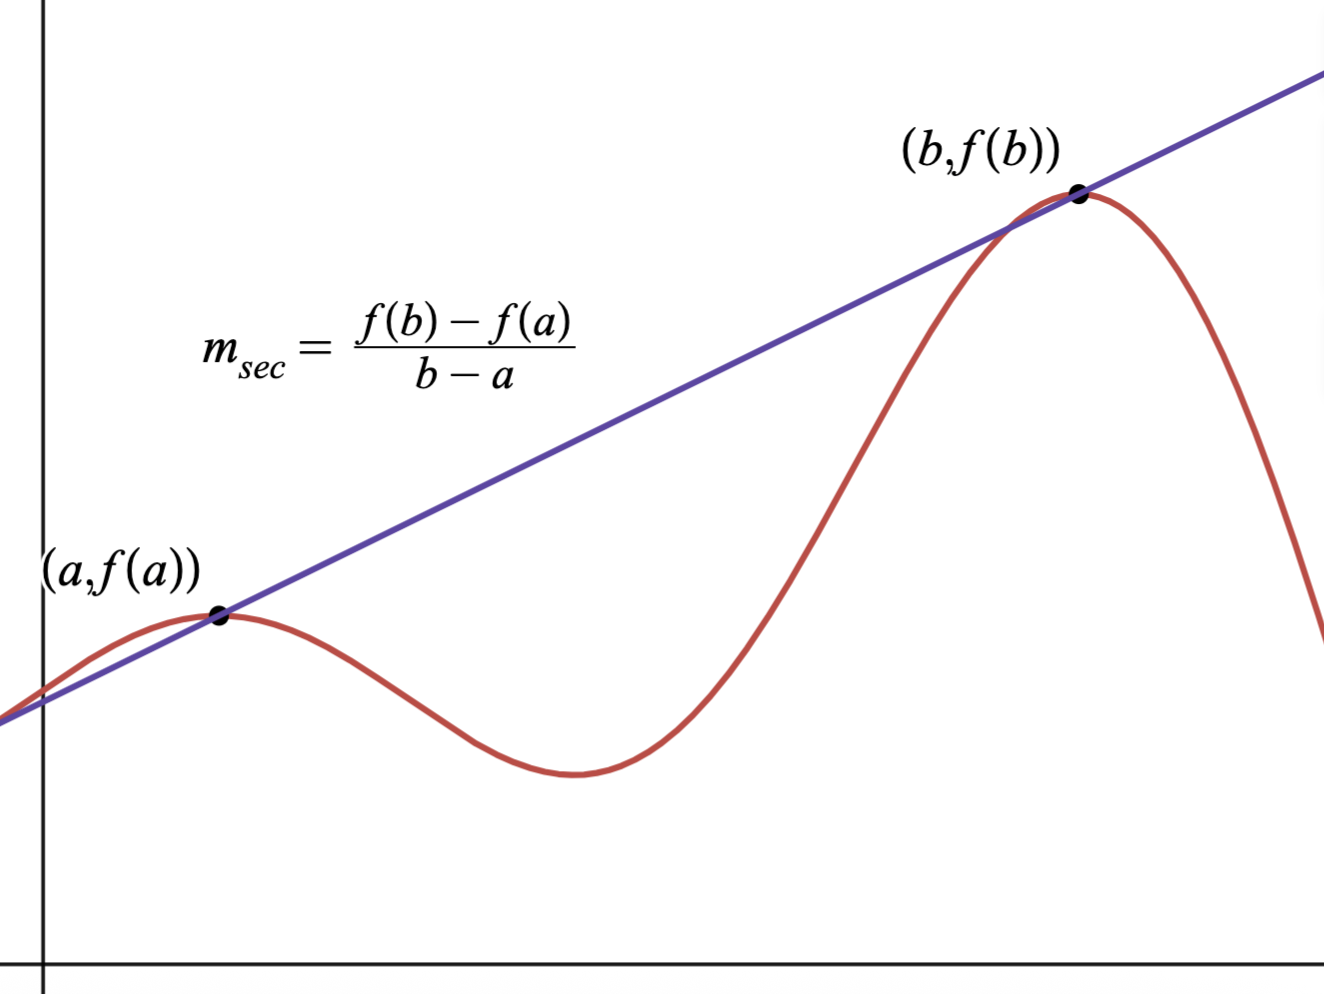
\includegraphics[width=4in]{./FunctionArithmeticGraphics/SecantLine.png}
%\end{center}

For the purposes of this section, consider a function $f$ defined over an interval containing $x$ and $x+\Delta x$ where $\Delta x \neq 0$. The average rate of change of $f$ over the interval $[x,x+\Delta x]$ is thus given by the formula:\footnote{assuming $\Delta x>0$;  otherwise, we  the interval is $[x+\Delta x, x]$.  We get the same formula for the difference quotient either way.}

\[ \dfrac{\Delta[f(x)]}{\Delta x} = \dfrac{f(x+\Delta x)-f(x)}{\Delta x}, \quad \Delta x \neq 0.\]

\medskip

Our aim in this section is to develop formulas which relate the rate of change of arithmetic combinations of functions to the rates of change of the constituent functions.   Our first step is to study the \index{difference operator}\index{operator ! difference}\textbf{difference operator}  `$\Delta$'  and study how it works with the standard arithmetic operations.  

\medskip

In general, if $u$ is some quantity which assumes two values in a particular order, say $u_{1}$ (the `first' or `initial' value) and $u_{2}$ (the `second' or `final' value), then $\Delta u = u_{2} - u_{1}$.  For example, if $u$ represents the temperature of an object before ($u_{1}$) heat is applied and after ($u_{2}$) heat is applied,  $\Delta u = u_{2} - u_{1}$ represents the increase in temperature of the object.

\medskip

 In the context of functions and rates of change, $u$ is the function $f$ defined on the interval $[x, x + \Delta x]$ with $u_{1} = f(x)$ and $u_{2} = f(x+\Delta x)$.  Here, $\Delta u = u_{2} - u_{1} = f(x+\Delta x) - f(x) = \Delta[f(x)]$.  
 
\medskip

Suppose we have two quantities, $u$ and $v$ with $\Delta u = u_{2} - u_{1}$ and $\Delta v = v_{2} - v_{1}$.   What do we mean by   $\Delta[u+v]$?  The initial value of the sum $u+v$ would be the sum of the initial values $u_{1} + v_{1}$. Likewise, the final value of the sum would be the sum of the final values $u_{2} + v_{2}$.  Hence:
 
\[ \begin{array}{rcl}

 \Delta[u+v] & = & (u_{2} + v_{2}) - (u_{1} + v_{1})   \\[8pt]
                                & = &   u_{2} + v_{2} - u_{1} - v_{1} \\[8pt]
                                & = &  (u_{2} - u_{1}) + (v_{2} - v_{1}) \\[8pt]
                                & = &  \Delta u + \Delta v  \\ \end{array} \]

A similar calculation gives $\Delta[u - v] = \Delta u - \Delta v$.

\medskip

Let's turn our attention to products. We have $\Delta[uv] = u_{2} \, v_{2} - u_{1} \, v_{1}$.  We'd like to express $\Delta[uv]$ in terms of $\Delta u$ and $\Delta v$ and there seems to be no way obvious way to do that.  We take to some geometric reasoning for inspiration.  Let's assume the all the quantities we're working with are positive.
\medskip

We imagine the product $u_{1} \, v_{1}$ as being the area of a rectangle with width $u_{1}$ and length $v_{1}$.  Likewise, the product $u_{2} \, v_{2}$ is the area of a (larger) rectangle with width $u_{2}$ and length $v_{2}$.

\medskip

\begin{center}

\begin{tabular}{cc}

\begin{mfpic}[35]{-1}{7}{-1}{4}
\tlabel[cc](-0.25,1){$u_{1}$}
\tlabel[cc](2,-0.25){$v_{1}$}
\tlabel[cc](2,1){$u_{1} \, v_{1}$}
\penwd{1.25pt}
\polyline{(0,0), (0,2), (4,2), (4,0), (0,0)}
\end{mfpic} 

& 

\begin{mfpic}[35]{-1}{7}{-1}{4}
\tlabel[cc](-0.25,1.5){$u_{2}$}
\tlabel[cc](3,-0.25){$v_{2}$}
\tlabel[cc](3,1.5){$u_{2} \, v_{2}$}
\penwd{1.25pt}
\polyline{(0,0), (0,3), (6,3), (6,0), (0,0)}
\end{mfpic}  \\

\end{tabular}

\end{center}

From $\Delta u = u_{2} - u_{1}$, we get $u_{2} = u_{1} + \Delta u$ and, likewise,  $v_{2} = v_{1} + \Delta v$.  Doing so allows us to decompose the larger rectangle into four smaller rectangles. 

\begin{center}


\begin{mfpic}[40]{-1}{7}{-1}{4}
\tlabel[cc](-0.3,2.5){$\Delta u$}
\tlabel[cc](-0.3,1){$u_{1}$}
\tlabel[cc](2,-0.25){$v_{1}$}
\tlabel[cc](5,-0.25){$\Delta v$}
\tlabel[cc](2,1){$u_{1} \, v_{1}$}
\tlabel[cc](2,2.5){$v_{1} \,  \Delta u $}
\tlabel[cc](5,1){$u_{1} \, \Delta v$}
\tlabel[cc](5,2.5){$\Delta u \,  \Delta v $}
\penwd{1.25pt}
\polyline{(0,0), (0,3), (6,3), (6,0), (0,0)}
\dashed \polyline{(0,2), (6,2)}
\dashed \polyline{(4,3), (4,0)}
\end{mfpic}  


\end{center}

Using this schematic, we see the area   $u_{2} \, v_{2}$ is the sum of the areas of four smaller rectangles:

\[ u_{2} \, v_{2}  = u_{1} \, v_{1} +  v_{1} \, \Delta u + u_{1} \, \Delta v + \Delta u \, \Delta v \]

Hence, $\Delta[uv]  = u_{2} \, v_{2} - u_{1} \, v_{1}  =  v_{1} \, \Delta u + u_{1} \, \Delta v +  \Delta u \, \Delta v$.

\medskip

To prove this formula holds in general, we can substitute $u_{2}  = u_{1} + \Delta u$ and $v_{2} = v_{1} + \Delta v$ into  $\Delta[uv] = u_{2} \, v_{2} - u_{1} \, v_{1}$ and simplify.  We leave the details to the reader.\footnote{Why not do this from the start, then?  Carl trained as a geometric topologist.}

\medskip

Next, we turn our attention to quotients.  We begin with: $\Delta \left[ \frac{u}{v} \right] = \frac{u_{2}}{v_{2}}  - \frac{u_{1}}{v_{1}}$.

\medskip

Instead of appealing to geometric reasoning here,\footnote{If you come up with or know of  a nice geometric argument and don't mind sharing, feel free to contact \href{mailto:carl@stitz-zeager.com}{\underline{Carl}}.} we take a cue from the previous discussion and substitute   $u_{2} = u_{1} + \Delta u$ and $v_{2} = v_{1} + \Delta v$ and set about getting a common denominator:

\[ \begin{array}{rcl}

\Delta\left[ \dfrac{u}{v}  \right]& = & \dfrac{u_{2}}{v_{2}} - \dfrac{u_{1}}{v_{1}}   \\[10pt]
                       & = &   \dfrac{ u_{1} + \Delta u}{ v_{1} + \Delta v} - \dfrac{u_{1}}{v_{1}}  \\[10pt]
                       & = &   \dfrac{(u_{1} + \Delta u) \, v_{1}}{(v_{1} + \Delta v) \, v_{1}} - \dfrac{u_{1} \, (v_{1} + \Delta v)}{v_{1} \,   (v_{1} + \Delta v) }\\[10pt]   
                            & = &   \dfrac{u_{1} \, v_{1}  + v_{1} \, \Delta u- u_{1} \, v_{1} - u_{1} \, \Delta v}{v_{1} \,  (v_{1} + \Delta v)}\\[10pt]   
                         & = &   \dfrac{ v_{1} \, \Delta u  - u_{1}  \, \Delta v}{v_{1} \,  (v_{1}  + \Delta v_{1})}\\
                       \end{array} \]
                       
We summarize these results in the following theorem.

\medskip

\colorbox{ResultColor}{\bbm

\begin{thm}  \label{functionarithmeticchange}  Suppose $\Delta u = u_{2} - u_{1}$ and $\Delta v = v_{2} - v_{1}$:
\begin{itemize}

\item  \textbf{The Sum Rule for Change:}   $\Delta[u+v] = \Delta u + \Delta v$

\item  \textbf{The Difference Rule for Change:}   $\Delta[u - v] = \Delta u - \Delta v$

\item  \textbf{The Product Rule for Change:}  $\Delta[uv]  =  v_{1} \, \Delta u + u_{1} \, \Delta v+  \Delta u \, \Delta v$

\item  \textbf{The Quotient Rule for Change:}  $\ds{ \Delta\left[ \dfrac{u}{v} \right] =  \dfrac{ v_{1} \, \Delta u  - u_{1}  \, \Delta v}{v_{1} \,  (v_{1}  + \Delta v_{1})}}$


\end{itemize}

\end{thm}

\ebm}

\medskip

In the following example, we use the Quotient Rule for Change to help approximate the \index{propagated error}\index{error ! propagated}\textbf{propagated error} when using measured quantities (with associated uncertainties) in calculations.\footnote{The adjective `propagated' here means than when we use measured quantities in calculations, the uncertainties in the measured quantities will produce, or `propagate' uncertainty in the calculated quantity.}

\medskip

\begin{ex}\label{densityexample} The density of a substance, $\rho$, is calculated by dividing its mass, $m$, by its volume, $V$:  $\rho = \frac{m}{V}$.  A scientist collects $5$ milliliters (mL) of a substance and determines its mass to be $68.2$ grams (g).  She computes the density as:  $\rho = \frac{68.2 \, \text{g}}{5 \, \text{mL}} = 13.64 \, \frac{\text{g}}{\text{mL}}$.

\medskip

Since every measurement in the lab has an associated uncertainty, she notes the pipet she used to measure the volume has an uncertainty of  $\pm 0.125$ mL and the balance she used to mass the substance has an uncertainty of  $\pm 0.01$ g.  This means the actual volume measurement can be anywhere from as low as  $5 - 0.125 = 4.875$ mL and as high as $5 + 0.125 = 5.125$ mL.  Likewise, the actual mass of the substance can be anywhere from $68.2 - 0.01 = 68.19$ g to $68.2+ 0.01 = 68.21$g.  Our goal is to help estimate the associated uncertainty  for the density, $\rho$.

\begin{enumerate}

\item Use Theorem \ref{functionarithmeticchange} to find an expression for the uncertainty in the volume $\Delta \rho$ produced as a result in the uncertainties in the measurements of mass, $\Delta m$, and volume, $\Delta V$.

\medskip

\item  Calculate $\frac{\Delta \rho}{\rho}$ and interpret your answer.

\end{enumerate}


{\bf Solution.}  

\begin{enumerate}

\item  In this scenario, we have two quantities, the volume, $V$ and the mass, $m$.  We'll take $V_{1}$ and $m_{1}$ to be the measured values of volume and mass, respectively, and use the uncertainties in each of the respective measurements as $\Delta V$ and $\Delta m$.  Since  $\Delta \rho = \Delta \left[ \frac{m}{V}\right]$, using the Quotient Rule from Theorem \ref{functionarithmeticchange} gives: \[ \Delta \rho =  \dfrac{ V_{1} \, \Delta m  - m_{1} \,  \Delta V }{V_{1} (V_{1} + \Delta V) }.\]

\item Substituting $V_{1} = 5$ mL, $m_{1} = 68.2$ g, $\Delta V =  \pm 0.125$ mL  and $\Delta m = \pm 0.01$ g gives:
  \[ \Delta \rho =  \dfrac{ (\pm 0.01 \, \text{g})  (5 \, \text{mL})  - (68.2 \, \text{g}) (\pm 0.125 \, \text{mL})} {(5 \, \text{mL})(5 \, \text{mL}  \pm 0.125 \, \text{mL})}.\]

Since we have no idea the exact value of each uncertainty, we need to make a judgement call as to which of the sign values,  `$\pm$' ,  to use.  To get the largest (most conservative) answer for $\Delta \rho$, we select the $\pm$ which generate the largest numerator and smallest denominator:

 \[ \Delta \rho =  \dfrac{ (+ 0.01 \, \text{g})  (5 \, \text{mL})  - (68.2 \, \text{g}) ( -  0.125 \, \text{mL})} {(5 \, \text{mL})(5 \, \text{mL}  -  0.125 \, \text{mL})}  = \frac{343 \, \text{g mL}}{975 \, \text{mL}^2} \approx  0.3517 \, \frac{\text{g}}{\text{mL}}\]
 
 Hence, $\frac{\Delta \rho}{\rho} \approx \frac{0.3517 \, \frac{\text{g}}{\text{mL}}}{13.64 \, \frac{\text{g}}{\text{mL}}}  \approx 0.0258 = 2.58 \%$.  
 
 \medskip
 
 We may interpret this as the uncertainties in the measurements for mass and volume in this situation could produce up to a $2.58 \%$ error in the calculated density,  \qed
\end{enumerate}

\end{ex}


In order to establish formulas for the average rate of change for  functions, we substitute $f(x)$ for $u_{1}$ and $g(x)$ for $v_{1}$ and divide each of the expressions in Theorem \ref{functionarithmeticchange} by $\Delta x$.  For example,  if we  to find an expression for the average rate of change of $fg$ in terms of $f$, $g$, and their respective average rates of change:

\[ \dfrac{\Delta[(fg)(x)]}{\Delta x} = \dfrac{ \Delta[f(x)]g(x) + f(x)\Delta[g(x)] + \Delta[f(x)]\Delta[g(x)]}{\Delta x} = \dfrac{\Delta[f(x)]}{\Delta x} \, g(x)  + f(x) \, \dfrac{\Delta[g(x)]}{\Delta x} + \dfrac{\Delta[f(x)]\Delta[g(x)]}{\Delta x}.\]

Note that with the last term, we may associate the `$\Delta x$' with either of the factors in the numerator: 

\[ \dfrac{\Delta[f(x)]\Delta[g(x)]}{\Delta x} = \dfrac{\Delta[f(x)]}{\Delta x} \, \Delta[g(x)] = \Delta[f(x)] \, \dfrac{\Delta[g(x)]}{\Delta x}.\]

Either way, we've managed to express the average rate of change of the function $fg$ in terms of the changes and rates of change of $f$ and $g$.  

  \medskip
  
In the result below, we abbreviate the average rate of change as `ARoC' for convenience.

\medskip

\colorbox{ResultColor}{\bbm

\begin{thm}  \label{functionarithmeticaroc}  Suppose $f$ and $g$ are functions defined on an interval containing $x$ and $x + \Delta x$, $\Delta x \neq 0$:
\begin{itemize}

\item  \textbf{The Sum Rule for ARoC:}   $\text{ARoC}[(f + g)(x)] = \text{ARoC}[f(x)] + \text{ARoC}[g(x)]$

\item  \textbf{The Difference Rule for ARoC:}   $\text{ARoC}[(f - g)(x)] = \text{ARoC}[f(x)] - \text{ARoC}[g(x)]$

\item  \textbf{The Product Rule for ARoC:}  

\[ \begin{array}{rcl}

\text{ARoC}[(fg)(x)]  & = & \text{ARoC}[f(x)] \, g(x) + f(x) \, \text{ARoC}[g(x)]  + \text{ARoC}[f(x)] \, g(x) \\[8pt]
                       & = &   \text{ARoC}[f(x)] \, g(x) + f(x) \, \text{ARoC}[g(x)]  + f(x) \, \text{ARoC}[g(x)]   \end{array} \]

\item  \textbf{The Quotient Rule for ARoC:}  \[\text{ARoC}\left[\left( \dfrac{f}{g} \right) (x) \right] = \dfrac{ \text{ARoC}[f(x)] \,  g(x)  - f(x) \, \text{ARoC}[g(x)]}{g(x) (g(x) + \Delta[g(x)])}\]


\end{itemize}

\end{thm}

\ebm}


\medskip

Our final example  revisits the scenario in Exercise \ref{newportaboycost} in Section \ref{GraphsofPolynomials}.  
\medskip

\begin{ex}\label{marginalsetupex}  The cost to produce $x$ `PortaBoy' handheld game systems is given by:  $C(x) = .03x^{3} - 4.5x^{2} + 225x + 250$ and the revenue generated by selling $x$ of the systems is given by $R(x) = -1.5x^2 + 250x$.


\medskip

\begin{enumerate}

\item  \label{costrevenuearcex} Find and interpret the average rate of change of $C$ and $R$ over the interval $[70,71]$.

\item   Use Theorem \ref{functionarithmeticaroc} to determine the average rate of change of the profit function, $P$ over the interval $[70, 71]$ using your answers to part \ref{costrevenuearcex}.  What does your answer suggest?  
\end{enumerate}

{\bf Solution.}

\begin{enumerate}

\item  We find $\text{ARoC}[C(x)] = \frac{C(71) - C(70)}{71-70} = \frac{4277.83 - 4240}{1} = 37.83$.  This means that as we move from producing $70$ to $71$ PortaBoy systems the cost will increase by $\$ 37.83$ per system.

\medskip

For revenue, we find  $\text{ARoC}[R(x)] = \frac{R(71) - R(70)}{71-70} = \frac{10188.5 - 10150}{1} = 38.5$.  This means that as we move from selling $70$ to $71$ PortaBoy systems, the revenue generated will increase by $\$ 38.5$ per system.

\medskip

\item  Since $P(x) = R(x) - C(x)$, the Difference Rule of Theorem \ref{functionarithmeticaroc} gives $\text{ARoC}[P(x)] = \text{ARoC}[R(x)] - \text{ARoC}[C(x)]$.  In this case, we'd get $\text{ARoC}[P(x)] =  38.5 - 37.83 = 0.67$.   This means as we move from producing and selling $70$ to $71$ PortaBoy systems, the profit generated will increase by just $67$ cents per system.  At this point, the increase in revenue is nearly balanced out by the increase in cost.  Since costs typically continue to rise as the number of items is produced while the revenue falls as we try to sell more items,\footnote{we've seen this before: to sell more, we lower the price which, in turn, lowers revenue \ldots} we are likely near a maximum point with the profit.  A quick check of the graph on Desmos confirms our suspicions.


\begin{center}
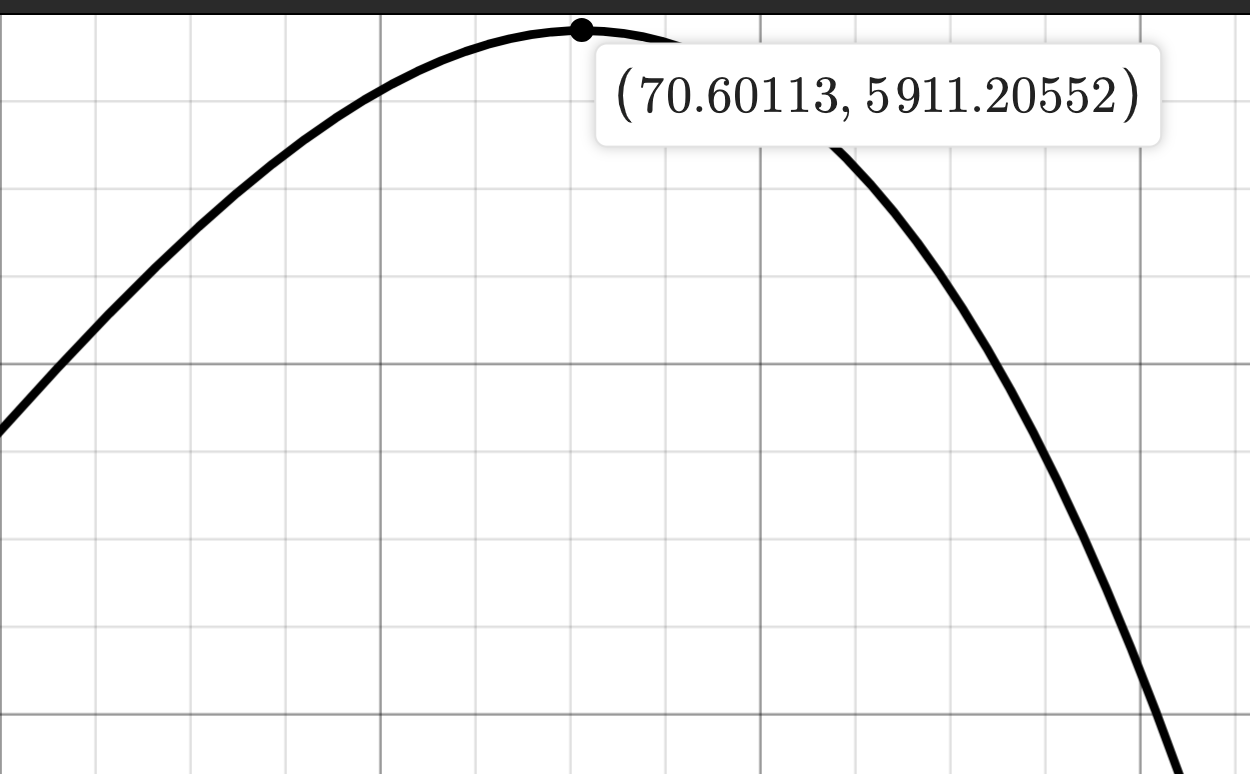
\includegraphics[width=4in]{./FunctionArithmeticGraphics/MaxProfitARoCEx.png}
\end{center}

\hfill  \qed

\end{enumerate}

\end{ex}

Note that in Example \ref{marginalsetupex}, since $\Delta x = 1$, the average rate of change for the cost moving from producing $70$ to $71$ systems, $ \frac{C(71) - C(70)}{71-70}$ is the same numerical value as the additional cost incurred by producing the $71$st system,  $C(71) - C(70)$.  The same goes for the revenue and profit calculations.  This is the concept of \index{marginal analysis}\index{analysis ! marginal}\textbf{marginal analysis} and will be explored further in the Exercises.
                       
                       
                       
\newpage

\subsection{Exercises}

\label{ExercisesforFunctionArithmetic}

In Exercises \ref{basicarithonefirst} - \ref{basicarithonelast}, use the pair of functions $f$ and $g$ to find the following values if they exist.

\begin{multicols}{3}
\begin{itemize}

\item  $(f+g)(2)$ 
\item  $(f-g)(-1)$
\item  $(g-f)(1)$

\end{itemize}
\end{multicols}

\begin{multicols}{3}
\begin{itemize}

\item  $(fg)\left(\frac{1}{2}\right)$
\item  $\left(\frac{f}{g}\right)(0)$
\item  $\left(\frac{g}{f}\right)\left(-2\right)$

\end{itemize}
\end{multicols}


\begin{multicols}{2}
\begin{enumerate}

\item  $f(x) = 3x+1$ and  $g(t) = 4-t$ \label{basicarithonefirst}
\item  $f(x) = x^2$ and $g(t) = -2t+1$

\setcounter{HW}{\value{enumi}}
\end{enumerate}
\end{multicols}

\begin{multicols}{2}
\begin{enumerate}
\setcounter{enumi}{\value{HW}}

\item  $f(x) = x^2 - x$ and  $g(t) = 12-t^2$
\item  $f(x) = 2x^3$ and $g(t) = -t^2-2t-3$

\setcounter{HW}{\value{enumi}}
\end{enumerate}
\end{multicols}

\begin{multicols}{2}
\begin{enumerate}
\setcounter{enumi}{\value{HW}}

\item  $f(x) = \sqrt{x+3}$ and  $g(t) = 2t-1$
\item  $f(x) = \sqrt{4-x}$ and $g(t) = \sqrt{t+2}$

\setcounter{HW}{\value{enumi}}
\end{enumerate}
\end{multicols}

\begin{multicols}{2}
\begin{enumerate}
\setcounter{enumi}{\value{HW}}

\item  $f(x) = 2x$ and  $g(t) = \dfrac{1}{2t+1}$
\item  $f(x) = x^2$ and $g(t) = \dfrac{3}{2t-3}$

\setcounter{HW}{\value{enumi}}
\end{enumerate}
\end{multicols}

\begin{multicols}{2}
\begin{enumerate}
\setcounter{enumi}{\value{HW}}

\item  $f(x) = x^2$ and  $g(t) = \dfrac{1}{t^2}$
\item  $f(x) = x^2+1$ and $g(t) = \dfrac{1}{t^2+1}$ \label{basicarithonelast}

\setcounter{HW}{\value{enumi}}
\end{enumerate}
\end{multicols}



Exercises \ref{arithfromgraphfirst} - \ref{arithfromgraphlast} refer to the functions $f$ and $g$ whose graphs are below. 

\begin{multicols}{2}

\begin{mfpic}[19]{-5}{5}{-5}{5}
\tlabel[cc](-3,0.5){\small $\left( -2, 0 \right)$}
\tlabel[cc](2.5,0.5){\small $\left(2, 0 \right)$}
\tlabel[cc](4,-3.5){\small $\left( 4, -3 \right)$}
\tlabel[cc](-4,-3.5){\small $\left(-4, -3 \right)$}
\tlabel[cc](1,3.5){\small $\left(0, 3 \right)$}
\axes
\tlabel[cc](5,-0.5){\scriptsize $x$}
\tlabel[cc](0.5,5){\scriptsize $y$}
\xmarks{-4,-3,-2,-1,1,2,3,4}
\ymarks{-4,-3,-2,-1,1,2,3,4}
\tlpointsep{5pt}
\scriptsize
\axislabels {x}{{$-4 \hspace{7pt}$} -4, {$-3 \hspace{7pt}$} -3, {$-2 \hspace{7pt}$} -2, {$-1 \hspace{7pt}$} -1, {$1$} 1, {$2$} 2, {$3$} 3, {$4$} 4}
\axislabels {y}{{$-4$} -4, {$-3$} -3, {$-2$} -2, {$-1$} -1, {$1$} 1, {$2$} 2, {$4$} 4}
\normalsize
\point[4pt]{(-2,0), (2,0), (4,-3), (-4,-3), (0,3)}
\penwd{1.25pt}
\function{-4,4,.1}{3*cos(3.14159265*x/4)}
\tcaption{$y = f(x)$}
\end{mfpic}


\begin{mfpic}[19]{-5}{5}{-5}{5}
\tlabel[cc](-4,-2.5){\small $\left( -4, -2 \right)$}
\tlabel[cc](-2,0.5){\small $\left(-1, 0 \right)$}
\tlabel[cc](-1,2){\small $\left( 0,2 \right)$}
\axes
\tlabel[cc](5,-0.5){\scriptsize $t$}
\tlabel[cc](0.5,5){\scriptsize $y$}
\xmarks{-4,-3,-2,-1,1,2,3,4}
\ymarks{-4,-3,-2,-1,1,2,3,4}
\tlpointsep{5pt}
\scriptsize
\axislabels {x}{{$-4 \hspace{7pt}$} -4, {$-3 \hspace{7pt}$} -3, {$-2 \hspace{7pt}$} -2, {$-1 \hspace{7pt}$} -1, {$1$} 1, {$2$} 2, {$3$} 3, {$4$} 4}
\axislabels {y}{{$-4$} -4, {$-3$} -3, {$-2$} -2, {$-1$} -1, {$1$} 1, {$4$} 4, {$3$} 3}
\normalsize
\point[4pt]{(-4,-2), (-1,0), (0,2)}
\penwd{1.25pt}
\polyline{(-4,-2), (-1,0), (0,2)}
\arrow \polyline{(0,2), (5,2)}
\tcaption{$y = g(t)$}
\end{mfpic}


\end{multicols}

\begin{multicols}{3}
\begin{enumerate}
\setcounter{enumi}{\value{HW}}

\item $(f + g)(-4)$ \label{arithfromgraphfirst}
\item $(f + g)(0)$
\item $(f- g)(4)$

\setcounter{HW}{\value{enumi}}
\end{enumerate}
\end{multicols}


\begin{multicols}{3}
\begin{enumerate}
\setcounter{enumi}{\value{HW}}

\item $(fg)(-4)$ 
\item $(fg)(-2)$
\item $(fg)(4)$

\setcounter{HW}{\value{enumi}}
\end{enumerate}
\end{multicols}

\enlargethispage{0.5in}

\begin{multicols}{3}
\begin{enumerate}
\setcounter{enumi}{\value{HW}}

\item $\left(\dfrac{f}{g}\right)(0)$
\item $\left(\dfrac{f}{g}\right)(2)$
\item $\left(\dfrac{g}{f}\right)(-1)$ 

\setcounter{HW}{\value{enumi}}
\end{enumerate}
\end{multicols}

\begin{enumerate}
\setcounter{enumi}{\value{HW}}

\item Find the domains of $f+g$, $f-g$,  $fg$, $\dfrac{f}{g}$ and $\dfrac{g}{f}$.  \label{arithfromgraphlast}

\setcounter{HW}{\value{enumi}}
\end{enumerate}

In Exercises \ref{reformarithfirst} - \ref{reformarithlast}, let $f$ be the function defined by \[f = \{(-3, 4), (-2, 2), (-1, 0), (0, 1), (1, 3), (2, 4), (3, -1)\}\] and let $g$ be the function defined by \[g = \{(-3, -2), (-2, 0), (-1, -4), (0, 0), (1, -3), (2, 1), (3, 2)\}\] Compute the indicated value if it exists.


\begin{multicols}{3}
\begin{enumerate}
\setcounter{enumi}{\value{HW}}

\item $(f + g)(-3)$ \label{reformarithfirst}
\item $(f - g)(2)$
\item $(fg)(-1)$

\setcounter{HW}{\value{enumi}}
\end{enumerate}
\end{multicols}

\begin{multicols}{3}
\begin{enumerate}
\setcounter{enumi}{\value{HW}}

\item $(g + f)(1)$
\item $(g - f)(3)$
\item $(gf)(-3)$

\setcounter{HW}{\value{enumi}}
\end{enumerate}
\end{multicols}

\begin{multicols}{3}
\begin{enumerate}
\setcounter{enumi}{\value{HW}}

\item $\left(\frac{f}{g}\right)(-2)$
\item $\left(\frac{f}{g}\right)(-1)$
\item $\left(\frac{f}{g}\right)(2)$

\setcounter{HW}{\value{enumi}}
\end{enumerate}
\end{multicols}

\begin{multicols}{3}
\begin{enumerate}
\setcounter{enumi}{\value{HW}}

\item $\left(\frac{g}{f}\right)(-1)$
\item $\left(\frac{g}{f}\right)(3)$
\item $\left(\frac{g}{f}\right)(-3)$ \label{reformarithlast}

\setcounter{HW}{\value{enumi}}
\end{enumerate}
\end{multicols}

In Exercises \ref{basicarithtwofirst} - \ref{basicarithtwolast}, use the pair of functions $f$ and $g$ to find the domain of the indicated function then find and simplify an expression for it.

\begin{multicols}{4}
\begin{itemize}

\item  $(f+g)(x)$
\item  $(f-g)(x)$
\item  $(fg)(x)$
\item  $\left(\frac{f}{g}\right)(x)$

\end{itemize}
\end{multicols}

\begin{multicols}{2}
\begin{enumerate}
\setcounter{enumi}{\value{HW}}

\item $f(x) = 2x+1$ and $g(x) = x-2$ \label{basicarithtwofirst}
\item $f(x) = 1-4x$ and $g(x) = 2x-1$

\setcounter{HW}{\value{enumi}}
\end{enumerate}
\end{multicols}

\begin{multicols}{2}
\begin{enumerate}
\setcounter{enumi}{\value{HW}}

\item $f(x) = x^2$ and $g(x) = 3x-1$
\item $f(x) = x^2-x$ and $g(x) = 7x$

\setcounter{HW}{\value{enumi}}
\end{enumerate}
\end{multicols}

\begin{multicols}{2}
\begin{enumerate}
\setcounter{enumi}{\value{HW}}

\item $f(x) = x^2-4$ and $g(x) = 3x+6$
\item $f(x) = -x^2+x+6$ and $g(x) = x^2-9$

\setcounter{HW}{\value{enumi}}
\end{enumerate}
\end{multicols}

\begin{multicols}{2}
\begin{enumerate}
\setcounter{enumi}{\value{HW}}

\item $f(x) = \dfrac{x}{2}$ and $g(x) = \dfrac{2}{x}$
\item $f(x) =x-1$ and $g(x) = \dfrac{1}{x-1}$

\setcounter{HW}{\value{enumi}}
\end{enumerate}
\end{multicols}

\begin{multicols}{2}
\begin{enumerate}
\setcounter{enumi}{\value{HW}}

\item $f(x) = x$ and $g(x) = \sqrt{x+1}$
\item $f(x) =\sqrt{x-5}$ and $g(x) = f(x) = \sqrt{x-5}$ \label{basicarithtwolast}

\setcounter{HW}{\value{enumi}}
\end{enumerate}
\end{multicols}

In Exercises \ref{decomposebasicfirst} - \ref{decomposebasiclast}, write the given function as a nontrivial decomposition of functions as directed.

\begin{enumerate}
\setcounter{enumi}{\value{HW}}

\item  For $p(z) = 4z-z^3$, find functions $f$ and $g$ so that $p=f-g$. \label{decomposebasicfirst}
\item  For $p(z) = 4z-z^3$, find functions $f$ and $g$ so that $p=f+g$.
\item  For $g(t) = 3t|2t-1|$, find functions $f$ and $h$  so that $g = fh$.
\item  For $r(x) = \dfrac{3-x}{x+1}$, find functions $f$ and $g$ so $r = \dfrac{f}{g}$.
\item  For $r(x) = \dfrac{3-x}{x+1}$, find functions $f$ and $g$ so $r = fg$. \label{decomposebasiclast}

\setcounter{HW}{\value{enumi}}
\end{enumerate}

\begin{enumerate}
\setcounter{enumi}{\value{HW}}

\item    Can $f(x) = x$ be decomposed as $f = g-h$ where $g(x) = x+\dfrac{1}{x}$ and $h(x) = \dfrac{1}{x}$?

\item   Discuss with your classmates how to phrase the quantities revenue and profit in Definition \ref{revenueprofitdefns} terms of function arithmetic as defined in Definition \ref{functionarithmeticdefn}.
 
\setcounter{HW}{\value{enumi}}
\end{enumerate}



\begin{enumerate}
\setcounter{enumi}{\value{HW}}

\item \label{posnegdecompexercise}  In this exercise, we explore decomposing a function into its positive and negative parts.  Given a function $f$, we define the \index{positive part of a function}\textbf{positive part} of $f$, denoted $f_{+}$ and \index{negative part of a function}\textbf{negative part} of $f$, denoted $f_{-}$ by:

\[ f_{+}(x) = \dfrac{f(x) + |f(x)|}{2}, \qquad \text{and} \qquad f_{-}(x) = \dfrac{f(x) - |f(x)|}{2}. \]

\begin{enumerate}

\item Using a graphing utility, graph each of the functions $f$ below along with $f_{+}$ and $f_{-}$.

\begin{multicols}{3}

\begin{itemize}

\item  $f(x) = x-3$

\item  $f(x) = x^2-x-6$

\item  $f(x) = 4x-x^3$

\end{itemize}

\end{multicols}

Why is $f_{+}$ called the `positive part' of $f$ and $f_{-}$ called the `negative part' of $f$?

\item Show that $f = f_{+} + f_{-}$.

\item Use Definition \ref{absolutevaluepiecewise} to rewrite the expressions for $f_{+}(x)$ and $f_{-}(x)$ as piecewise defined functions.

\end{enumerate}  

\setcounter{HW}{\value{enumi}}
\end{enumerate}


\begin{enumerate}
\setcounter{enumi}{\value{HW}}

\item  Let $U$ be the unit step function defined in Exercise \ref{unitstepexercise} in Section \ref{ConstantandLinearFunctions}.  For each function $f(t)$ below:

\begin{itemize}

\item  Write $(Uf)(t)$ as a piecewise-defined function.

\item  Graph $y = f(t)$ and $y = (Uf)(t)$.

\end{itemize}

\begin{multicols}{3}

\begin{enumerate}

\item $f(t) = t-3$



\item  $f(t) = |t+2|$



\item  $f(t) =(t-1)^2$



\setcounter{HW}{\value{enumii}}

\end{enumerate}

\end{multicols}

\begin{multicols}{3}

\begin{enumerate}

\setcounter{enumii}{\value{HW}}

\item  $f(t) =(t+1)^{-1}$



\item  $f(t) = \sqrt[3]{t-1}$ \vphantom{ $f(t) =(t+1)^{-1}$}



\item  $f(t) = (t-2)^{\frac{2}{3}}$ \vphantom{ $f(t) =(t+1)^{-1}$}



\setcounter{HW}{\value{enumii}}

\end{enumerate}

\end{multicols}

\begin{enumerate}

\setcounter{enumii}{\value{HW}}

\item  Write a general formula for $(Uf)(t)$ for a function $f$.  (Assume the domain of $f$ is $(-\infty, \infty)$.)



\item  Explain how to obtain the graph of $y=(Uf)(t)$ from $y=f(t)$.


\item The function $U(t)$ is used to model a change in state from `off' to `on' (like flipping a light switch.)  How does this relate to your observations?



\item  Use the graph of $y=f(t)$ below to graph $y=(Uf)(t)$.

\begin{center}

\begin{mfpic}[15]{-5}{5}{-4}{4}
\tlabel[cc](-2.25,-3.5){\scriptsize $\left( -2, -3 \right)$}
\tlabel[cc](2,3.5){\scriptsize $\left(2, 3 \right)$}
\tlabel[cc](-4.25,0.5){\scriptsize $\left(-4, 0 \right)$}
\tlabel[cc](0.75,-0.5){\scriptsize $\left(0, 0 \right)$}
\axes
\tcaption{ \scriptsize$y = f(t)$}
\tlabel[cc](5,-0.5){\scriptsize $t$}
\tlabel[cc](0.5,4){\scriptsize $y$}
\xmarks{-4,-3,-2,-1,1,2,3,4}
\ymarks{-3,-2,-1,1,2,3}
\tlpointsep{5pt}
\scriptsize
\axislabels {x}{ {$-3 \hspace{7pt}$} -3, {$-2 \hspace{7pt}$} -2, {$-1 \hspace{7pt}$} -1, {$2$} 2, {$3$} 3, {$4$} 4}
\axislabels {y}{ {$-3$} -3, {$-2$} -2,  {$1$} 1, {$2$} 2, {$3$} 3}
\normalsize
\penwd{1.25pt}
\function{-4,2,.1}{3*sin(3.14159265*x/4)}
\point[4pt]{(-2,-3), (2,3),  (-4,0), (0,0)}
\end{mfpic}

\end{center}


\end{enumerate}

\item Use Example \ref{densityexample} as a guide to help find the following uncertainties.  

\begin{enumerate}

\item  A chemist combines the solutions from two graduated cylinders into a beaker.  The volume of the first solution, $A$, an acid,  is read as $A_{1} = 101 \pm 0.5$ milliliters (mL). The volume of the second solution,  a base, $B$,  is measured to be $B_{1} = 16 \pm 0.5$ mL.    Estimate the percent propagated error in calculating the volume of the combined solution as $V = A_{1} + B_{1} = 101 + 16 = 117$ mL.

\item  A student measures the length, $\ell$, and width, $w$,  of a piece of paper.  They find  $\ell_{1} = 280 \pm 0.5$ millimeters (mm) $w_{1} = 216 \pm 0.5$ mm.    Estimate the percent propagated error in calculating the area of the piece of paper as $A = \ell_{1} \, w_{1} = 280 \times 216 = 60480 \, \text{mm}^2$.

\item  An airplane passenger  observers a car travel a distance $d_{1} = 1320 \pm 2$ feet (ft) in time $t_{1}  = 15 \pm 0.5$ seconds (s).  Estimate the percent propagated error in calculating the speed of the car as $v = \frac{d_{1}}{t_{1}} = \frac{1320}{15} = 88 \, \frac{\text{ft}}{\text{s}}$.

\end{enumerate}

\item\label{AverageCostMarginalCostExercise} Let us return to Example \ref{marginalsetupex} where  $C(x) = .03x^{3} - 4.5x^{2} + 225x + 250$ denotes the cost, in dollars,  of producing $x$ PortaBoy game systems. Recall the \index{average cost}\index{cost ! average}\textbf{average cost}\footnote{First mentioned in Definition \ref{averagecostprofit} in Section \ref{IntroRational}.} is defined as $\overline{C}(x) = \frac{C(x)}{x}$, $x > 0$,  is the cost per item.

\begin{enumerate}

\item\label{ACexercise1} Find and interpret $\overline{C}(75)$.

\item\label{MCexercise1}  Define  the \index{marginal cost}\index{cost ! marginal}\textbf{marginal cost} $MC(x) = C(x+1) - C(x)$.   Find and interpret $MC(75)$.

\item  How do your answers to parts \ref{ACexercise1} and \ref{MCexercise1} compare?

\item Graph $y = \overline{C}(x)$ with help from a graphing utility.  What is happening graphically near $x = 75$?

\item  Use Theorem \ref{functionarithmeticaroc} to show that, in general, $\text{ARoC}[ \overline{C}(x)] = 0$ when $MC(x) = \overline{C}(x)$.

\smallskip

\textbf{HINT:}  Note that, by definition, $MC(x) = C(x+1) - C(x) = \Delta[C(x)]$ when $\Delta x = 1$.  

\smallskip

Hence,  $\text{ARoC}[C(x)] = \frac{\Delta[C(x)]}{\Delta x} = \frac{\Delta[C(x)]}{1} = \Delta[C(x)] = MC(x)$ in this case \ldots 

\end{enumerate}

\setcounter{HW}{\value{enumi}}

\end{enumerate}


\newpage

\subsection{Answers}

\begin{enumerate}

\item For  $f(x) = 3x+1$ and $g(x) = 4-x$

\begin{multicols}{3}
\begin{itemize}

\item  $(f+g)(2) = 9$
\item  $(f-g)(-1) = -7$
\item  $(g-f)(1) = -1$

\end{itemize}
\end{multicols}

\begin{multicols}{3}
\begin{itemize}

\item  $(fg)\left(\frac{1}{2}\right) = \frac{35}{4}$
\item  $\left(\frac{f}{g}\right)(0) = \frac{1}{4}$
\item  $\left(\frac{g}{f}\right)\left(-2\right) = -\frac{6}{5}$

\end{itemize}
\end{multicols}

\item For  $f(x) = x^2$ and $g(x) = -2x+1$

\begin{multicols}{3}
\begin{itemize}

\item  $(f+g)(2) = 1$
\item  $(f-g)(-1) = -2$
\item  $(g-f)(1) = -2$

\end{itemize}
\end{multicols}

\begin{multicols}{3}
\begin{itemize}

\item  $(fg)\left(\frac{1}{2}\right) = 0$
\item  $\left(\frac{f}{g}\right)(0) = 0$
\item  $\left(\frac{g}{f}\right)\left(-2\right) = \frac{5}{4}$

\end{itemize}
\end{multicols}

\item For  $f(x) = x^2 - x$ and  $g(x) = 12-x^2$

\begin{multicols}{3}
\begin{itemize}

\item  $(f+g)(2) = 10$
\item  $(f-g)(-1) = -9$
\item  $(g-f)(1) = 11$

\end{itemize}
\end{multicols}

\begin{multicols}{3}
\begin{itemize}

\item  $(fg)\left(\frac{1}{2}\right) = -\frac{47}{16}$
\item  $\left(\frac{f}{g}\right)(0) = 0$
\item  $\left(\frac{g}{f}\right)\left(-2\right) = \frac{4}{3}$

\end{itemize}
\end{multicols}

\item For $f(x) = 2x^3$ and  $g(x) = -x^2-2x-3$

\begin{multicols}{3}
\begin{itemize}

\item  $(f+g)(2) = 5$
\item  $(f-g)(-1) = 0$
\item  $(g-f)(1) = -8$

\end{itemize}
\end{multicols}

\begin{multicols}{3}
\begin{itemize}

\item  $(fg)\left(\frac{1}{2}\right) = -\frac{17}{16}$
\item  $\left(\frac{f}{g}\right)(0) = 0$
\item  $\left(\frac{g}{f}\right)\left(-2\right) = \frac{3}{16}$

\end{itemize}
\end{multicols}

\item For $f(x) = \sqrt{x+3}$ and  $g(x) = 2x-1$

\begin{multicols}{3}
\begin{itemize}

\item  $(f+g)(2) = 3+\sqrt{5}$
\item  $(f-g)(-1) = 3+\sqrt{2}$
\item  $(g-f)(1) = -1$

\end{itemize}
\end{multicols}

\begin{multicols}{3}
\begin{itemize}

\item  $(fg)\left(\frac{1}{2}\right) = 0$
\item  $\left(\frac{f}{g}\right)(0) = -\sqrt{3}$
\item  $\left(\frac{g}{f}\right)\left(-2\right) = -5$

\end{itemize}
\end{multicols}

\item For $f(x) = \sqrt{4-x}$ and $g(x) = \sqrt{x+2}$

\begin{multicols}{3}
\begin{itemize}

\item  $(f+g)(2) = 2+\sqrt{2}$
\item  $(f-g)(-1) = -1+\sqrt{5}$
\item  $(g-f)(1) = 0$

\end{itemize}
\end{multicols}

\begin{multicols}{3}
\begin{itemize}

\item  $(fg)\left(\frac{1}{2}\right) = \frac{\sqrt{35}}{2}$
\item  $\left(\frac{f}{g}\right)(0) = \sqrt{2}$
\item  $\left(\frac{g}{f}\right)\left(-2\right) = 0$

\end{itemize}
\end{multicols}

\newpage

\item For  $f(x) = 2x$ and  $g(x) = \frac{1}{2x+1}$

\begin{multicols}{3}
\begin{itemize}

\item  $(f+g)(2) = \frac{21}{5}$
\item  $(f-g)(-1) = -1$
\item  $(g-f)(1) = -\frac{5}{3}$

\end{itemize}
\end{multicols}

\begin{multicols}{3}
\begin{itemize}

\item  $(fg)\left(\frac{1}{2}\right) = \frac{1}{2}$
\item  $\left(\frac{f}{g}\right)(0) = 0$
\item  $\left(\frac{g}{f}\right)\left(-2\right) = \frac{1}{12}$

\end{itemize}
\end{multicols}

\item For  $f(x) = x^2$ and $g(x) = \frac{3}{2x-3}$

\begin{multicols}{3}
\begin{itemize}

\item  $(f+g)(2) = 7$
\item  $(f-g)(-1) = \frac{8}{5}$
\item  $(g-f)(1) = -4$

\end{itemize}
\end{multicols}

\begin{multicols}{3}
\begin{itemize}

\item  $(fg)\left(\frac{1}{2}\right) = -\frac{3}{8}$
\item  $\left(\frac{f}{g}\right)(0) = 0$
\item  $\left(\frac{g}{f}\right)\left(-2\right) = -\frac{3}{28}$

\end{itemize}
\end{multicols}

\item For  $f(x) = x^2$ and $g(x) = \frac{1}{x^2}$

\begin{multicols}{3}
\begin{itemize}

\item  $(f+g)(2) =\frac{17}{4}$
\item  $(f-g)(-1) = 0$
\item  $(g-f)(1) = 0$

\end{itemize}
\end{multicols}

\begin{multicols}{3}
\begin{itemize}

\item  $(fg)\left(\frac{1}{2}\right) =1$
\item  $\left(\frac{f}{g}\right)(0)$ is undefined.
\item  $\left(\frac{g}{f}\right)\left(-2\right) = \frac{1}{16}$

\end{itemize}
\end{multicols}

\item For  $f(x) = x^2+1$ and $g(x) = \frac{1}{x^2+1}$

\begin{multicols}{3}
\begin{itemize}

\item  $(f+g)(2) =\frac{26}{5}$
\item  $(f-g)(-1) = \frac{3}{2}$
\item  $(g-f)(1) = -\frac{3}{2}$

\end{itemize}
\end{multicols}

\begin{multicols}{3}
\begin{itemize}

\item  $(fg)\left(\frac{1}{2}\right) =1$
\item  $\left(\frac{f}{g}\right)(0) = 1$
\item  $\left(\frac{g}{f}\right)\left(-2\right) = \frac{1}{25}$

\end{itemize}
\end{multicols}

\setcounter{HW}{\value{enumi}}
\end{enumerate}

\begin{multicols}{3}
\begin{enumerate}
\setcounter{enumi}{\value{HW}}

\item $(f + g)(-4) = -5$   
\item $(f + g)(0) = 5$
\item $(f-g)(4) = -5$

\setcounter{HW}{\value{enumi}}
\end{enumerate}
\end{multicols}


\begin{multicols}{3}
\begin{enumerate}
\setcounter{enumi}{\value{HW}}

\item $(fg)(-4) = 6$ 
\item $(fg)(-2) = 0$
\item $(fg)(4) = -6$

\setcounter{HW}{\value{enumi}}
\end{enumerate}
\end{multicols}

\enlargethispage{0.5in}

\begin{multicols}{3}
\begin{enumerate}
\setcounter{enumi}{\value{HW}}

\item $\left(\dfrac{f}{g}\right)(0) = \dfrac{3}{2}$
\item $\left(\dfrac{f}{g}\right)(2) =  0$
\item $\left(\dfrac{g}{f}\right)(-1) = 0$ 

\setcounter{HW}{\value{enumi}}
\end{enumerate}
\end{multicols}

\begin{enumerate}
\setcounter{enumi}{\value{HW}}

\item The domains of $f+g$, $f-g$ and $fg$ are all $[-4,4]$.  The domain of $\frac{f}{g}$ is $[-4, -1) \cup (-1,4]$ and the domain of $\frac{g}{f}$ is $[-4, -2) \cup (-2,2) \cup (2, 4]$.

\setcounter{HW}{\value{enumi}}
\end{enumerate}


\begin{multicols}{3}
\begin{enumerate}
\setcounter{enumi}{\value{HW}}

\item $(f + g)(-3) = 2$
\item $(f - g)(2) = 3$
\item $(fg)(-1) = 0$

\setcounter{HW}{\value{enumi}}
\end{enumerate}
\end{multicols}

\begin{multicols}{3}
\begin{enumerate}
\setcounter{enumi}{\value{HW}}

\item $(g + f)(1) = 0$
\item $(g - f)(3) = 3$
\item $(gf)(-3) = -8$

\setcounter{HW}{\value{enumi}}
\end{enumerate}
\end{multicols}

\begin{multicols}{3}
\begin{enumerate}
\setcounter{enumi}{\value{HW}}

\item $\left(\frac{f}{g}\right)(-2)$ does not exist
\item $\left(\frac{f}{g}\right)(-1) = 0$
\item $\left(\frac{f}{g}\right)(2) = 4$

\setcounter{HW}{\value{enumi}}
\end{enumerate}
\end{multicols}

\begin{multicols}{3}
\begin{enumerate}
\setcounter{enumi}{\value{HW}}

\item $\left(\frac{g}{f}\right)(-1)$ does not exist
\item $\left(\frac{g}{f}\right)(3) = -2$ 
\item $\left(\frac{g}{f}\right)(-3) = -\frac{1}{2}$ 

\setcounter{HW}{\value{enumi}}
\end{enumerate}
\end{multicols}

\newpage

\begin{enumerate}
\setcounter{enumi}{\value{HW}}

\item For $f(x) = 2x+1$ and $g(x) = x-2$

\begin{multicols}{2}

\begin{itemize}

\item $(f+g)(x) = 3x-1$ \\
      Domain: $(-\infty, \infty)$
      
      \vfill
      
      \columnbreak
      
\item $(f-g)(x) = x+3$ \\
      Domain:  $(-\infty, \infty)$


\end{itemize}

\end{multicols}

\begin{multicols}{2}

\begin{itemize}

\item $(fg)(x) = 2x^2-3x-2$ \\
      Domain: $(-\infty, \infty)$
      
      \vfill
      
      \columnbreak
      
\item $\left(\frac{f}{g}\right)(x) = \frac{2x+1}{x-2}$ \\
      Domain:  $(-\infty, 2) \cup (2, \infty)$


\end{itemize}

\end{multicols}

\item For $f(x) = 1-4x$ and $g(x) = 2x-1$

\begin{multicols}{2}

\begin{itemize}

\item $(f+g)(x) = -2x$ \\
      Domain: $(-\infty, \infty)$
      
      \vfill
      
      \columnbreak
      
\item $(f-g)(x) = 2-6x$ \\
      Domain:  $(-\infty, \infty)$


\end{itemize}

\end{multicols}

\begin{multicols}{2}

\begin{itemize}

\item $(fg)(x) = -8x^2+6x-1$ \\
      Domain: $(-\infty, \infty)$
      
      \vfill
      
      \columnbreak
      
\item $\left(\frac{f}{g}\right)(x) = \frac{1-4x}{2x-1}$ \\
      Domain:  $\left(-\infty, \frac{1}{2} \right) \cup \left(\frac{1}{2}, \infty \right)$


\end{itemize}

\end{multicols}


\item For $f(x) = x^2$ and $g(x) = 3x-1$

\begin{multicols}{2}

\begin{itemize}

\item $(f+g)(x) = x^2+3x-1$ \\
      Domain: $(-\infty, \infty)$
      
      \vfill
      
      \columnbreak
      
\item $(f-g)(x) = x^2-3x+1$ \\
      Domain:  $(-\infty, \infty)$


\end{itemize}

\end{multicols}

\begin{multicols}{2}

\begin{itemize}

\item $(fg)(x) = 3x^3-x^2$ \\
      Domain: $(-\infty, \infty)$
      
      \vfill
      
      \columnbreak
      
\item $\left(\frac{f}{g}\right)(x) = \frac{x^2}{3x-1}$ \\
      Domain:  $\left(-\infty, \frac{1}{3} \right) \cup \left(\frac{1}{3}, \infty \right)$


\end{itemize}

\end{multicols}

\item For $f(x) = x^2-x$ and $g(x) = 7x$

\begin{multicols}{2}

\begin{itemize}

\item $(f+g)(x) = x^2+6x$ \\
      Domain: $(-\infty, \infty)$
      
      \vfill
      
      \columnbreak
      
\item $(f-g)(x) = x^2-8x$ \\
      Domain:  $(-\infty, \infty)$


\end{itemize}

\end{multicols}

\begin{multicols}{2}

\begin{itemize}

\item $(fg)(x) = 7x^3-7x^2$ \\
      Domain: $(-\infty, \infty)$
      
      \vfill
      
      \columnbreak
      
\item $\left(\frac{f}{g}\right)(x) = \frac{x-1}{7}$ \\
      Domain:  $\left(-\infty, 0 \right) \cup \left(0, \infty \right)$


\end{itemize}

\end{multicols}


\item For $f(x) = x^2-4$ and $g(x) = 3x+6$

\begin{multicols}{2}

\begin{itemize}

\item $(f+g)(x) = x^2+3x+2$ \\
      Domain: $(-\infty, \infty)$
      
      \vfill
      
      \columnbreak
      
\item $(f-g)(x) = x^2-3x-10$ \\
      Domain:  $(-\infty, \infty)$


\end{itemize}

\end{multicols}

\begin{multicols}{2}

\begin{itemize}

\item $(fg)(x) = 3x^3+6x^2-12x-24$ \\
      Domain: $(-\infty, \infty)$
      
      \vfill
      
      \columnbreak
      
\item $\left(\frac{f}{g}\right)(x) = \frac{x-2}{3}$ \\
      Domain:  $\left(-\infty, -2 \right) \cup \left(-2, \infty \right)$


\end{itemize}

\end{multicols}

\newpage

\item For $f(x) = -x^2+x+6$ and $g(x) = x^2-9$

\begin{multicols}{2}

\begin{itemize}

\item $(f+g)(x) = x-3$ \\
      Domain: $(-\infty, \infty)$
      
      \vfill
      
      \columnbreak
      
\item $(f-g)(x) = -2x^2+x+15$ \\
      Domain:  $(-\infty, \infty)$


\end{itemize}

\end{multicols}

\begin{multicols}{2}

\begin{itemize}

\item $(fg)(x) = -x^4+x^3+15x^2-9x-54$ \\
      Domain: $(-\infty, \infty)$
      
      \vfill
      
      \columnbreak
      
\item $\left(\frac{f}{g}\right)(x) = -\frac{x+2}{x+3}$ \\
      Domain:  $\left(-\infty, -3 \right) \cup \left(-3, 3 \right) \cup (3, \infty)$


\end{itemize}

\end{multicols}


\item For  $f(x) = \frac{x}{2}$ and $g(x) = \frac{2}{x}$

\begin{multicols}{2}

\begin{itemize}

\item $(f+g)(x) = \frac{x^2+4}{2x}$ \\
      Domain: $(-\infty, 0) \cup (0, \infty)$
      
      \vfill
      
      \columnbreak
      
\item $(f-g)(x) = \frac{x^2-4}{2x}$ \\
      Domain:  $(-\infty,0) \cup (0, \infty)$


\end{itemize}

\end{multicols}

\begin{multicols}{2}

\begin{itemize}

\item $(fg)(x) = 1$ \\
      Domain: $(-\infty,0) \cup (0, \infty)$
      
      \vfill
      
      \columnbreak
      
\item $\left(\frac{f}{g}\right)(x) = \frac{x^2}{4}$ \\
      Domain: $(-\infty,0) \cup (0, \infty)$


\end{itemize}

\end{multicols}



\item For   $f(x) =x-1$ and $g(x) = \frac{1}{x-1}$

\begin{multicols}{2}

\begin{itemize}

\item $(f+g)(x) = \frac{x^2-2x+2}{x-1}$ \\
      Domain: $(-\infty, 1) \cup (1, \infty)$
      
      \vfill
      
      \columnbreak
      
\item $(f-g)(x) = \frac{x^2-2x}{x-1}$ \\
      Domain:  $(-\infty,1) \cup (1, \infty)$


\end{itemize}

\end{multicols}

\begin{multicols}{2}

\begin{itemize}

\item $(fg)(x) = 1$ \\
      Domain: $(-\infty,1) \cup (1, \infty)$
      
      \vfill
      
      \columnbreak
      
\item $\left(\frac{f}{g}\right)(x) =x^2-2x+1$ \\
      Domain: $(-\infty,1) \cup (1, \infty)$


\end{itemize}

\end{multicols}


\item For   $f(x) =x$ and $g(x) = \sqrt{x+1}$

\begin{multicols}{2}

\begin{itemize}

\item $(f+g)(x) = x+\sqrt{x+1}$ \\
      Domain: $[-1,\infty)$
      
      \vfill
      
      \columnbreak
      
\item $(f-g)(x) = x-\sqrt{x+1}$ \\
       Domain: $[-1,\infty)$


\end{itemize}

\end{multicols}

\begin{multicols}{2}

\begin{itemize}

\item $(fg)(x) = x\sqrt{x+1}$ \\
       Domain: $[-1,\infty)$
      
      \vfill
      
      \columnbreak
      
\item $\left(\frac{f}{g}\right)(x) =\frac{x}{\sqrt{x+1}}$ \\
       Domain: $(-1,\infty)$


\end{itemize}

\end{multicols}

\item For   $f(x) = \sqrt{x-5}$ and $g(x) = f(x) = \sqrt{x-5}$

\begin{multicols}{2}

\begin{itemize}

\item $(f+g)(x) = 2\sqrt{x-5}$ \\
      Domain: $[5,\infty)$
      
      \vfill
      
      \columnbreak
      
\item $(f-g)(x) =0$ \\
       Domain: $[5,\infty)$


\end{itemize}

\end{multicols}

\begin{multicols}{2}

\begin{itemize}

\item $(fg)(x) =x-5$ \\
       Domain: $[5,\infty)$
      
      \vfill
      
      \columnbreak
      
\item $\left(\frac{f}{g}\right)(x) =1$ \\
       Domain: $(5,\infty)$


\end{itemize}

\end{multicols}

\setcounter{HW}{\value{enumi}}
\end{enumerate}

\newpage

\begin{enumerate}
\setcounter{enumi}{\value{HW}}

\item One solution is $f(z) = 4z$ and $g(z) = z^3$. 
\item One solution is $f(z) = 4z$ and $g(z) = - z^3$. 
\item One solution is  $f(t) = 3t$ and $h(t) = |2t-1|$ 
\item One solution is $f(x) = 3-x$ and $g(x) = x+1$.  
\item  One solution is $f(x) = 3-x$ and $g(x) = (x+1)^{-1}$.  

\setcounter{HW}{\value{enumi}}
\end{enumerate}

\begin{enumerate}
\setcounter{enumi}{\value{HW}}

\item No.  The equivalence does not hold when $x = 0$.

\setcounter{HW}{\value{enumi}}
\end{enumerate}

\begin{enumerate}
\setcounter{enumi}{\value{HW}}
\addtocounter{enumi}{1}
\item  \begin{enumerate}  

\addtocounter{enumii}{1}

\item $(f_{+} + f_{-})(x) =  f_{+}(x) + f_{-}(x) = \dfrac{f(x) + |f(x)|}{2} + \dfrac{f(x) - |f(x)|}{2} = \dfrac{2f(x)}{2} = f(x)$.

\item   \[ f_{+}(x)  =  \begin{mycases} 
    0 &  \text{if $f(x) < 0$} \\
      f(x) & \text{if $f(x)  \geq 0$} \\
   \end{mycases},  \qquad    f_{-}(x)  =  \begin{mycases} 
    f(x) &  \text{if $f(x) < 0$} \\
      0 & \text{if $f(x)  \geq 0$} \\
   \end{mycases} \]

\end{enumerate}


\setcounter{HW}{\value{enumi}}
\end{enumerate}




\begin{enumerate}
\setcounter{enumi}{\value{HW}}

\item  $~$


\begin{enumerate}

\item $(Uf)(t) =  \begin{cases} 
  0  &  \text{if $t < 0$, } \\
    t-3  & \text{if $t \geq 0$.} \\
   \end{cases}$


\begin{multicols}{2}

\begin{mfpic}[12]{-5}{5}{-5}{5}
\axes
\tlabel[cc](5,-0.5){\scriptsize $t$}
\tlabel[cc](0.5,5){\scriptsize $y$}
\xmarks{-4,-3,-2,-1,1,2,3,4}
\ymarks{-4,-3,-2, -1, 1,2,3,4}
\tlpointsep{4pt}
\scriptsize
\axislabels {x}{ {$-4 \hspace{7pt}$} -4, {$-3 \hspace{7pt}$} -3, {$-2 \hspace{7pt}$} -2, {$-1 \hspace{7pt}$} -1, {$1$} 1, {$2$} 2, {$3$} 3, {$4$} 4}
\axislabels {y}{{$-1$} -1, {$-2$} -2, {$-4$} -4,{$-3$} -3,  {$1$} 1, {$2$} 2, {$3$} 3, {$4$} 4}
\penwd{1.25pt}
\arrow \reverse \arrow \polyline{( -2,-5), (5,2)}
\tcaption{ \scriptsize$y = f(t)$}
\normalsize
\end{mfpic} 


\begin{mfpic}[12]{-5}{5}{-5}{5}
\axes
\tlabel[cc](5,-0.5){\scriptsize $t$}
\tlabel[cc](0.5,5){\scriptsize $y$}
\xmarks{-4,-3,-2,-1,1,2,3,4}
\ymarks{-4,-3,-2, -1, 1,2,3,4}
\tlpointsep{4pt}
\scriptsize
\axislabels {x}{ {$-4 \hspace{7pt}$} -4, {$-3 \hspace{7pt}$} -3, {$-2 \hspace{7pt}$} -2, {$-1 \hspace{7pt}$} -1, {$1$} 1, {$2$} 2, {$3$} 3, {$4$} 4}
\axislabels {y}{{$-1$} -1,{$-2$} -2,{$-3$} -3,{$-4$} -4,{$1$} 1, {$2$} 2, {$3$} 3, {$4$} 4}
\penwd{1.25pt}
\arrow \reverse \polyline{( -5,0), (0,0)}
\arrow \polyline{(0,-3), (5,2)}
\point[4pt]{(0,-3)}
\pointfillfalse
\point[4pt]{(0,0)}
\tcaption{ \scriptsize$y = (Uf)(t)$}
\normalsize
\end{mfpic} 
\end{multicols}


\newpage 


\item $(Uf)(t) =  \begin{cases} 
   0  &  \text{if $t < 0$, } \\
    |t+2|  = t+2 & \text{if $t \geq 0$.} \\
   \end{cases}$



\begin{multicols}{2}

\begin{mfpic}[12]{-5}{5}{-5}{5}
\axes
\tlabel[cc](5,-0.5){\scriptsize $t$}
\tlabel[cc](0.5,5){\scriptsize $y$}
\xmarks{-4,-3,-2,-1,1,2,3,4}
\ymarks{-4,-3,-2, -1, 1,2,3,4}
\tlpointsep{4pt}
\scriptsize
\axislabels {x}{ {$-4 \hspace{7pt}$} -4, {$-3 \hspace{7pt}$} -3, {$-2 \hspace{7pt}$} -2, {$-1 \hspace{7pt}$} -1, {$1$} 1, {$2$} 2, {$3$} 3, {$4$} 4}
\axislabels {y}{{$-1$} -1, {$-2$} -2, {$-4$} -4,{$-3$} -3,  {$1$} 1, {$2$} 2, {$3$} 3, {$4$} 4}
\penwd{1.25pt}
\arrow \reverse \arrow \polyline{( -5,3), (-2,0), (3,5)}
\tcaption{ \scriptsize$y = f(t)$}
\normalsize
\end{mfpic} 


\begin{mfpic}[12]{-5}{5}{-5}{5}
\axes
\tlabel[cc](5,-0.5){\scriptsize $t$}
\tlabel[cc](0.5,5){\scriptsize $y$}
\xmarks{-4,-3,-2,-1,1,2,3,4}
\ymarks{-4,-3,-2, -1, 1,2,3,4}
\tlpointsep{4pt}
\scriptsize
\axislabels {x}{ {$-4 \hspace{7pt}$} -4, {$-3 \hspace{7pt}$} -3, {$-2 \hspace{7pt}$} -2, {$-1 \hspace{7pt}$} -1, {$1$} 1, {$2$} 2, {$3$} 3, {$4$} 4}
\axislabels {y}{{$-1$} -1,{$-2$} -2,{$-3$} -3,{$-4$} -4,{$1$} 1, {$2$} 2, {$3$} 3, {$4$} 4}
\penwd{1.25pt}
\arrow \reverse \polyline{( -5,0), (0,0)}
\arrow \polyline{(0,2), (3,5)}
\point[4pt]{(0,2)}
\pointfillfalse
\point[4pt]{(0,0)}
\tcaption{ \scriptsize$y = (Uf)(t)$}
\normalsize
\end{mfpic} 
\end{multicols}





\item  $(Uf)(t) =  \begin{cases} 
   0  &  \text{if $t < 0$, } \\
   (t-1)^2 & \text{if $t \geq 0$.} \\
   \end{cases}$



\begin{multicols}{2}

\begin{mfpic}[12]{-5}{5}{-5}{5}
\axes
\tlabel[cc](5,-0.5){\scriptsize $t$}
\tlabel[cc](0.5,5){\scriptsize $y$}
\xmarks{-4,-3,-2,-1,1,2,3,4}
\ymarks{-4,-3,-2, -1, 1,2,3,4}
\tlpointsep{4pt}
\scriptsize
\axislabels {x}{ {$-4 \hspace{7pt}$} -4, {$-3 \hspace{7pt}$} -3, {$-2 \hspace{7pt}$} -2, {$-1 \hspace{7pt}$} -1, {$1$} 1, {$2$} 2, {$3$} 3, {$4$} 4}
\axislabels {y}{{$-1$} -1, {$-2$} -2, {$-4$} -4,{$-3$} -3,  {$1$} 1, {$2$} 2, {$3$} 3, {$4$} 4}
\penwd{1.25pt}
\arrow \reverse \arrow \function{-1.2, 3.2, 0.1}{(x-1)**2}
\tcaption{ \scriptsize$y = f(t)$}
\normalsize
\end{mfpic} 


\begin{mfpic}[12]{-5}{5}{-5}{5}
\axes
\tlabel[cc](5,-0.5){\scriptsize $t$}
\tlabel[cc](0.5,5){\scriptsize $y$}
\xmarks{-4,-3,-2,-1,1,2,3,4}
\ymarks{-4,-3,-2, -1, 1,2,3,4}
\tlpointsep{4pt}
\scriptsize
\axislabels {x}{ {$-4 \hspace{7pt}$} -4, {$-3 \hspace{7pt}$} -3, {$-2 \hspace{7pt}$} -2, {$-1 \hspace{7pt}$} -1, {$1$} 1, {$2$} 2, {$3$} 3, {$4$} 4}
\axislabels {y}{{$-1$} -1,{$-2$} -2,{$-3$} -3,{$-4$} -4,{$1$} 1, {$2$} 2, {$3$} 3, {$4$} 4}
\penwd{1.25pt}
\arrow \reverse \polyline{( -5,0), (0,0)}
\arrow \function{0, 3.2, 0.1}{(x-1)**2}
\point[4pt]{(0,1)}
\pointfillfalse
\point[4pt]{(0,0)}
\tcaption{ \scriptsize$y = (Uf)(t)$}
\normalsize
\end{mfpic} 
\end{multicols}




\setcounter{HW}{\value{enumii}}

\end{enumerate}



\begin{enumerate}

\setcounter{enumii}{\value{HW}}

\item  $(Uf)(t) =  \begin{cases} 
  0  &  \text{if $t < 0$, $t \neq -1$ } \\
   (t+1)^{-1} & \text{if $t \geq 0$.} \\
   \end{cases}$
   



\begin{multicols}{2}

\begin{mfpic}[12]{-5}{5}{-5}{5}
\axes
\tlabel[cc](5,-0.5){\scriptsize $t$}
\tlabel[cc](0.5,5){\scriptsize $y$}
\xmarks{-4,-3,-2,-1,1,2,3,4}
\ymarks{-4,-3,-2, -1, 1,2,3,4}
\tlpointsep{4pt}
\scriptsize
\axislabels {x}{ {$-4 \hspace{7pt}$} -4, {$-3 \hspace{7pt}$} -3, {$-2 \hspace{7pt}$} -2, {$-1 \hspace{7pt}$} -1, {$1$} 1, {$2$} 2, {$3$} 3, {$4$} 4}
\axislabels {y}{{$-1$} -1, {$-2$} -2, {$-4$} -4,{$-3$} -3,  {$1$} 1, {$2$} 2, {$3$} 3, {$4$} 4}
\dashed \polyline{(-1,-5), (-1,5)}
\penwd{1.25pt}
\arrow \reverse  \arrow \function{-5, -1.25, 0.1}{(x+1)**(-1)}
\arrow  \reverse \arrow \function{-0.75, 5,  0.1}{(x+1)**(-1)}
\tcaption{ \scriptsize$y = f(t)$}
\normalsize
\end{mfpic} 


\begin{mfpic}[12]{-5}{5}{-5}{5}
\axes
\tlabel[cc](5,-0.5){\scriptsize $t$}
\tlabel[cc](0.5,5){\scriptsize $y$}
\xmarks{-4,-3,-2,-1,1,2,3,4}
\ymarks{-4,-3,-2, -1, 1,2,3,4}
\tlpointsep{4pt}
\scriptsize
\axislabels {x}{ {$-4 \hspace{7pt}$} -4, {$-3 \hspace{7pt}$} -3, {$-2 \hspace{7pt}$} -2, {$-1 \hspace{7pt}$} -1, {$1$} 1, {$2$} 2, {$3$} 3, {$4$} 4}
\axislabels {y}{{$-1$} -1,{$-2$} -2,{$-3$} -3,{$-4$} -4,{$1$} 1, {$2$} 2, {$3$} 3, {$4$} 4}
\penwd{1.25pt}
\arrow \reverse  \polyline{( -5,0), (0,0)}
\arrow \function{0, 5, 0.1}{(x+1)**(-1)}
\point[4pt]{(0,1)}
\pointfillfalse
\point[4pt]{(0,0), (-1,0)}
\tcaption{ \scriptsize$y = (Uf)(t)$  - note the hole at $(-1,0)$}
\normalsize
\end{mfpic} 
\end{multicols}



\item $(Uf)(t) =  \begin{cases} 
   0  &  \text{if $t < 0$, } \\
    \sqrt[3]{t-1} & \text{if $t \geq 0$.} \\
   \end{cases}$
   
   \begin{multicols}{2}

\begin{mfpic}[12]{-5}{5}{-5}{5}
\axes
\tlabel[cc](5,-0.5){\scriptsize $t$}
\tlabel[cc](0.5,5){\scriptsize $y$}
\xmarks{-4,-3,-2,-1,1,2,3,4}
\ymarks{-4,-3,-2, -1, 1,2,3,4}
\tlpointsep{4pt}
\scriptsize
\axislabels {x}{ {$-4 \hspace{7pt}$} -4, {$-3 \hspace{7pt}$} -3, {$-2 \hspace{7pt}$} -2, {$-1 \hspace{7pt}$} -1, {$1$} 1, {$2$} 2, {$3$} 3, {$4$} 4}
\axislabels {y}{{$-1$} -1, {$-2$} -2, {$-4$} -4,{$-3$} -3,  {$1$} 1, {$2$} 2, {$3$} 3, {$4$} 4}
\penwd{1.25pt}
\arrow \reverse \arrow \parafcn{-1.8, 1.5, 0.1}{(1+t**3, t)}
\tcaption{ \scriptsize$y = f(t)$}
\normalsize
\end{mfpic} 


\begin{mfpic}[12]{-5}{5}{-5}{5}
\axes
\tlabel[cc](5,-0.5){\scriptsize $t$}
\tlabel[cc](0.5,5){\scriptsize $y$}
\xmarks{-4,-3,-2,-1,1,2,3,4}
\ymarks{-4,-3,-2, -1, 1,2,3,4}
\tlpointsep{4pt}
\scriptsize
\axislabels {x}{ {$-4 \hspace{7pt}$} -4, {$-3 \hspace{7pt}$} -3, {$-2 \hspace{7pt}$} -2, {$-1 \hspace{7pt}$} -1, {$1$} 1, {$2$} 2, {$3$} 3, {$4$} 4}
\axislabels {y}{{$-1$} -1,{$-2$} -2,{$-3$} -3,{$-4$} -4,{$1$} 1, {$2$} 2, {$3$} 3, {$4$} 4}
\penwd{1.25pt}
\arrow \reverse \polyline{( -5,0), (0,0)}
 \arrow \parafcn{-1, 1.5, 0.1}{(1+t**3, t)}
\point[4pt]{(0,-1)}
\pointfillfalse
\point[4pt]{(0,0)}
\tcaption{ \scriptsize$y = (Uf)(t)$}
\normalsize
\end{mfpic} 
\end{multicols}



\item  $(Uf)(t) =  \begin{cases} 
   0  &  \text{if $t < 0$, } \\
   (t-2)^{\frac{2}{3}} & \text{if $t \geq 0$.} \\
   \end{cases}$
   
   
   \begin{multicols}{2}

\begin{mfpic}[12]{-5}{5}{-5}{5}
\axes
\tlabel[cc](5,-0.5){\scriptsize $t$}
\tlabel[cc](0.5,5){\scriptsize $y$}
\xmarks{-4,-3,-2,-1,1,2,3,4}
\ymarks{-4,-3,-2, -1, 1,2,3,4}
\tlpointsep{4pt}
\scriptsize
\axislabels {x}{ {$-4 \hspace{7pt}$} -4, {$-3 \hspace{7pt}$} -3, {$-2 \hspace{7pt}$} -2, {$-1 \hspace{7pt}$} -1, {$1$} 1, {$2$} 2, {$3$} 3, {$4$} 4}
\axislabels {y}{{$-1$} -1, {$-2$} -2, {$-4$} -4,{$-3$} -3,  {$1$} 1, {$2$} 2, {$3$} 3, {$4$} 4}
\penwd{1.25pt}
\arrow \reverse \arrow \parafcn{-1.9, 1.4, 0.1}{(2+t**3, t**2)}
\tcaption{ \scriptsize$y = f(t)$}
\normalsize
\end{mfpic} 


\begin{mfpic}[12]{-5}{5}{-5}{5}
\axes
\tlabel[cc](5,-0.5){\scriptsize $t$}
\tlabel[cc](0.5,5){\scriptsize $y$}
\xmarks{-4,-3,-2,-1,1,2,3,4}
\ymarks{-4,-3,-2, -1, 1,2,3,4}
\tlpointsep{4pt}
\scriptsize
\axislabels {x}{ {$-4 \hspace{7pt}$} -4, {$-3 \hspace{7pt}$} -3, {$-2 \hspace{7pt}$} -2, {$-1 \hspace{7pt}$} -1, {$1$} 1, {$2$} 2, {$3$} 3, {$4$} 4}
\axislabels {y}{{$-1$} -1,{$-2$} -2,{$-3$} -3,{$-4$} -4,{$1$} 1, {$2$} 2, {$3$} 3, {$4$} 4}
\penwd{1.25pt}
\arrow \reverse \polyline{( -5,0), (0,0)}
\arrow \parafcn{-1.25, 1.44, 0.1}{(2+t**3, t**2)}
\point[4pt]{(0,1.587)}
\pointfillfalse
\point[4pt]{(0,0)}
\tcaption{ \scriptsize$y = (Uf)(t)$}
\normalsize
\end{mfpic} 
\end{multicols}




\setcounter{HW}{\value{enumii}}

\end{enumerate}



\begin{enumerate}

\setcounter{enumii}{\value{HW}}

\item   $(Uf)(t) =  \begin{cases} 
   0  &  \text{if $t < 0$, } \\
    f(t)  & \text{if $t \geq 0$} \\
   \end{cases}$

\item  The graph of $(Uf)(t)$ is $y=0$ for $t < 0$ and $y=f(t)$ for $t \geq 0$.

\item The unit step function keeps the function `off' until $t=0$ then turns the function `on' for $t \geq 0$.


\item  $~$

\begin{center}

\begin{mfpic}[12]{-5}{5}{-4}{4}
\tlabel[cc](2,3.5){\scriptsize $\left(2, 3 \right)$}
\tlabel[cc](0.75,-0.5){\scriptsize $\left(0, 0 \right)$}
\axes
\tcaption{ \scriptsize$y = (Uf)(t)$}
\tlabel[cc](5,-0.5){\scriptsize $t$}
\tlabel[cc](0.5,4){\scriptsize $y$}
\xmarks{-4,-3,-2,-1,1,2,3,4}
\ymarks{-3,-2,-1,1,2,3}
\tlpointsep{5pt}
\scriptsize
\axislabels {x}{  {$-4 \hspace{7pt}$} -4,{$-3 \hspace{7pt}$} -3, {$-2 \hspace{7pt}$} -2, {$-1 \hspace{7pt}$} -1, {$2$} 2, {$3$} 3, {$4$} 4}
\axislabels {y}{ {$-3$} -3, {$-2$} -2,  {$1$} 1, {$2$} 2, {$3$} 3}
\normalsize
\penwd{1.25pt}
\function{0,2,.1}{3*sin(3.14159265*x/4)}
\polyline{(-4,0), (0,0)}
\point[4pt]{(2,3),  (-4,0), (0,0)}
\end{mfpic}

\end{center}


\end{enumerate}

\item \begin{enumerate}

\item   $\Delta V = \Delta[ A +B ] = \Delta A  + \Delta B = \pm 0.5 \, \text{mL} + \pm 0.5 \, \text{mL} = \pm 1 \, \text{mL}$.  

$\frac{\Delta V}{V} = \pm \frac{1}{117} \approx 0.85 \, \%$.

\item   $\Delta A = \Delta [ \ell w] = w_{1} \Delta \ell  + \ell_{1} \Delta w + \Delta \ell \Delta w =  (216 \, \text{mm})(\pm 0.5 \, \text{mm}) +  (280 \, \text{mm})(\pm 0.5 \, \text{mm})  + (\pm 0.5 \, \text{mm})(\pm 0.5 \, \text{mm}) = \pm 248.25 \, \text{mm}^2$. 

 $\frac{\Delta A}{A} = \pm \frac{248.25}{60480} \approx 0.41\, \%$

\item $\Delta v =  \Delta \left[ \frac{d}{t} \right] = \frac{t_{1} \, \Delta d  - d_{1} \,  \Delta t }{t_{1} (t_{1} + \Delta t) } = \frac{ (15 \, \text{s})(\pm 2 \, \text{ft})  - (1320 \, \text{ft})(\pm 0.5 \, \text{s})}{ (15 \, \text{s})  (15 \pm  0.5 \, \text{s}) } = \pm \frac{92}{29} \, \frac{\text{ft}}{\text{s}} \approx 3.17 \, \frac{\text{ft}}{\text{s}}$.  

$\frac{\Delta v}{v} \approx  \pm \frac{3.17}{88} \approx 3.60 \, \%$


\end{enumerate}

\item \begin{enumerate}  \item $\overline{C}(75) \approx 59.58$.  When making $75$ systems, the cost per system is approximately $\$ 59.58$.

\item $MC(75) = C(76) - C(75) = 58.53$.  It costs an additional $\$ 58.53$ to make the $76$th system.

\item  $\overline{C}(75)$ and $MC(75)$ appear to be `pretty close.'

\item  The graph $y = \overline{C}(x)$  has a local (absolute) minimum right near $x = 75$.

\item  Per Theorem \ref{functionarithmeticaroc}, since 

  \[ \begin{array}{lcrl}
  
  \text{ARoC}[ \overline{C}(x)] = \text{ARoC}\left[\dfrac{C(x)}{x}   \right] & = & \dfrac{ \text{ARoC}[C(x)] \,  x  - C(x)  \, \text{ARoC}[x]}{x (x + \Delta x)} & \\[10pt]  
   & = & \dfrac{ \text{ARoC}[C(x)] \,  x  - C(x)(1) }{x (x +\Delta x)} & \text{Since $\text{ARoC}[x] = \frac{\Delta x}{ \Delta x} = 1$}\\[10pt]  \end{array}\]

If $\text{ARoC}[ \overline{C}(x)]  = 0$, then the numerator,  $\text{ARoC}[C(x)] \,  x  - C(x) = 0$.  Solving for $\text{ARoC}[C(x)]$ , we get  $\text{ARoC}[C(x)] = \frac{C(x)}{x} = \overline{C}(x)$.  If we are working with a whole number of items, the smallest meaningful value of $\Delta x$ is $1$, in which case $\text{ARoC}[C(x)]  = MC(x)$.  Hence,  $\text{ARoC}[ \overline{C}(x)] = 0$ when $MC(x) = \overline{C}(x)$, that is, when  the marginal cost and average cost are the same.  At this point, the graph of $y = \overline{C}(x)$ levels off (at a minumum.)\footnote{We'll have more to say on this after Section \ref{AppDerivatives} in Exercise \ref{MinimizeAverageCostProofExercise}.} Can you reason why this creates a minimum?



\setcounter{HW}{\value{enumi}}

\end{enumerate}

\setcounter{HW}{\value{enumi}}
\end{enumerate}








\closegraphsfile